% Final-draft preview for Chapters I--V.
% TODO: Replace placeholders with official university, faculty, author, and supervisor information.
\documentclass[12pt,a4paper,oneside]{report}

\usepackage{iftex}
\ifPDFTeX
  \usepackage[utf8]{inputenc}
  \usepackage[T5]{fontenc}
  \usepackage[vietnamese]{babel}
\else
  \usepackage{fontspec}
  \usepackage[vietnamese]{babel}
  \setmainfont{Times New Roman}
\fi

\usepackage{geometry}
\geometry{left=3.0cm,right=2.5cm,top=2.5cm,bottom=2.5cm}

\usepackage{amsmath,amssymb,amsfonts}
\usepackage{graphicx}
\usepackage{booktabs}
\usepackage{array}
\usepackage{multirow}
\usepackage{tabularx}
\usepackage{algorithm}
\usepackage{algpseudocode}
\usepackage[numbers,sort&compress]{natbib}
\usepackage[hidelinks]{hyperref}
\usepackage{xcolor}
\usepackage{enumitem}
\usepackage{caption}
\usepackage{float}

\graphicspath{{../../results/publication_figures/}{figures/}}
\emergencystretch=3em

\renewcommand{\chaptername}{Chương}
\renewcommand{\contentsname}{Mục lục}
\renewcommand{\bibname}{Tài liệu tham khảo}
\setlist[itemize]{leftmargin=1.2cm}

\title{
  \textbf{Học tăng cường đa tác tử cho mạng UAV-IoT hỗ trợ chống gây nhiễu với truyền thông backscatter cảm hứng RF-powered}\\
  \vspace{0.5cm}
  \large Bản thảo LaTeX hoàn thiện sơ bộ
}
\author{
  Sinh viên thực hiện: \textbf{TODO: Họ và tên sinh viên}\\
  Mã số sinh viên: \textbf{TODO: MSSV}\\
  Giảng viên hướng dẫn: \textbf{TODO: Họ và tên giảng viên}
}
\date{
  Trường/Viện: \textbf{TODO: Tên trường}\\
  Khoa/Bộ môn: \textbf{TODO: Tên khoa/bộ môn}\\
  \vspace{0.3cm}
  \today
}

\begin{document}

\maketitle
\chapter*{Tóm tắt}
\addcontentsline{toc}{chapter}{Tóm tắt}

Mạng IoT hỗ trợ bởi thiết bị bay không người lái (UAV) là một hướng tiếp cận linh hoạt cho thu thập dữ liệu trong các khu vực thiếu hạ tầng hoặc có thiết bị IoT năng lượng hạn chế. Tuy nhiên, khi xuất hiện jammer di động, UAV phải đồng thời quyết định vị trí di chuyển, thiết bị cần phục vụ và chế độ truyền thông trong điều kiện kênh thay đổi, hàng đợi biến động và rủi ro gây nhiễu. Bài toán càng phức tạp hơn khi xem xét các thiết bị IoT có khả năng harvest, backscatter cảm hứng RF-powered và truyền active.

Báo cáo này nghiên cứu bài toán điều khiển UAV-IoT chống gây nhiễu bằng học tăng cường sâu và học tăng cường đa tác tử. Thiết lập đánh giá cuối cùng sử dụng cấu hình mô phỏng đã triển khai gồm 2 UAV, 15 thiết bị IoT và 1 jammer di động, với frame length bằng 10 và episode length bằng 200. Trên cấu hình này, giao diện hành động nguyên thủy có 864 hành động, gây khó khăn cho Flat DDQN. Vì vậy, báo cáo sử dụng một giao diện hành động phân cấp gồm 10 hành động mức cao, sau đó một bộ thực thi dựa trên quy tắc ánh xạ hành động mức cao về hành động nguyên thủy.

Các kết quả Phase 3 cho thấy Flat DDQN gặp khó khăn với giao diện 864 hành động, trong khi Hierarchical DDQN chứng minh rằng trừu tượng hóa hành động làm bài toán khả học hơn. Phương pháp cuối cùng được lựa chọn là QMIX-Hierarchical, trong đó mỗi UAV chọn hành động mức cao từ quan sát cục bộ, còn mạng trộn QMIX sử dụng trạng thái toàn cục và phần thưởng chung trong huấn luyện. QMIX-Hierarchical đạt hành vi hợp tác ổn định qua ba seed và cải thiện các chỉ số liên quan đến gây nhiễu/công bằng so với Hierarchical DDQN đơn chạy. Báo cáo diễn giải các kết quả một cách thận trọng: QMIX không được khẳng định vượt Hierarchical DDQN về thông lượng trung bình, fairness chưa được giải quyết triệt để, và mô hình backscatter là trừu tượng mức hệ thống chứ không phải xác thực vật lý đầy đủ.

\clearpage

\tableofcontents
\listoffigures
\listoftables
\clearpage

\chapter{Giới thiệu}

\section{Bối cảnh nghiên cứu}

Internet vạn vật (Internet of Things, IoT) ngày càng được triển khai trong các môi trường phân tán, khó tiếp cận hoặc thiếu hạ tầng truyền thông cố định. Trong các bối cảnh này, thiết bị bay không người lái (Unmanned Aerial Vehicle, UAV) có thể đóng vai trò như nút thu thập dữ liệu, trạm phủ sóng tạm thời hoặc nền tảng phục vụ linh hoạt cho các thiết bị IoT \cite{uav_iot_survey_todo}. Khả năng di chuyển của UAV giúp hệ thống thích nghi với phân bố thiết bị, trạng thái hàng đợi và chất lượng kênh theo thời gian.

Nhiều thiết bị IoT có năng lượng hạn chế nên không thể phụ thuộc hoàn toàn vào truyền chủ động công suất cao. Các cơ chế RF-powered và backscatter-inspired tạo ra một hướng tiếp cận hấp dẫn ở mức hệ thống: thiết bị có thể harvest năng lượng khi kênh sơ cấp bận, truyền backscatter khi có điều kiện phù hợp, hoặc truyền active khi có đủ năng lượng. Báo cáo này sử dụng cách mô hình hóa backscatter ở mức trừu tượng hệ thống, không khẳng định đây là mô hình vật lý ambient-backscatter đầy đủ.

\section{Vấn đề gây nhiễu trong mạng UAV-IoT}

Gây nhiễu vô tuyến làm tăng nhiễu tại bộ thu, suy giảm SINR và làm tăng xác suất truyền thất bại. Trong mạng UAV-IoT, tác động này không chỉ làm giảm thông lượng mà còn làm tăng rơi gói, kéo dài hàng đợi và làm mất công bằng phục vụ giữa các thiết bị. Khi jammer có khả năng di động, vùng rủi ro nhiễu thay đổi theo thời gian; UAV phải cân bằng giữa việc di chuyển đến gần IoT, tránh jammer và chọn chế độ truyền phù hợp.

Bài toán vì vậy có tính động và tổ hợp: tại mỗi frame, mỗi UAV phải quyết định di chuyển, chọn IoT mục tiêu và chọn chế độ truyền thông. Các heuristic đơn giản có thể mạnh trong một số điều kiện, nhưng thường chỉ tối ưu một khía cạnh như khoảng cách, SINR, active-only hoặc backscatter-only. Điều này tạo động lực cho các chính sách học thích nghi.

\section{Động lực sử dụng học tăng cường đa tác tử}

Học tăng cường (Reinforcement Learning, RL) phù hợp với điều khiển mạng động vì chính sách có thể học từ tương tác với môi trường và tối ưu tín hiệu thưởng dài hạn \cite{sutton2018reinforcement}. Các phương pháp DQN và Double DQN mở rộng Q-learning bằng mạng nơ-ron sâu, giúp xử lý không gian trạng thái lớn và hành động rời rạc \cite{mnih2015dqn,vanhasselt2016ddqn}.

Tuy nhiên, trong hệ nhiều UAV, mỗi UAV có quan sát và hành động riêng nhưng mục tiêu là hiệu quả toàn mạng. Điều này làm cho học tăng cường đa tác tử (Multi-Agent Reinforcement Learning, MaDRL) phù hợp hơn so với cách xem toàn bộ hệ thống như một tác tử đơn. QMIX là một lựa chọn tự nhiên cho bài toán hợp tác có hành động rời rạc, phần thưởng chung, quan sát cục bộ và trạng thái toàn cục dùng trong huấn luyện \cite{rashid2018qmix}.

\section{Khoảng trống nghiên cứu}

Các nghiên cứu về RF-powered/backscatter thường tập trung vào lập lịch, offloading hoặc tối ưu chế độ truyền trong các thiết lập tương đối riêng lẻ. Các nghiên cứu UAV-IoT thường nhấn mạnh quỹ đạo, vùng phủ hoặc thu thập dữ liệu. Trong khi đó, ít công trình kết hợp đồng thời các yếu tố sau trong cùng một thiết lập mô phỏng: nhiều UAV phục vụ IoT dị thể, jammer di động, lựa chọn harvest/backscatter/active, trừu tượng hóa hành động phân cấp và học phối hợp bằng QMIX.

Khoảng trống chính của đề tài là giao diện điều khiển. Nếu để tác tử học trực tiếp trên hành động nguyên thủy, không gian hành động trong Scenario 4 có kích thước 864. Kết quả thực nghiệm cho thấy Flat DDQN gặp khó khăn với giao diện này. Do đó, báo cáo tập trung vào việc kết hợp trừu tượng hóa hành động 10 mức cao với QMIX-Hierarchical.

\section{Mục tiêu nghiên cứu}

Các mục tiêu chính gồm:

\begin{itemize}
  \item mô hình hóa môi trường UAV-IoT có jammer di động, hàng đợi IoT, năng lượng thiết bị và các chế độ idle/harvest/backscatter/active;
  \item sử dụng backscatter-inspired/RF-powered abstraction để mô tả quyết định truyền thông của IoT năng lượng thấp;
  \item đánh giá Flat DDQN, Hierarchical DDQN và QMIX-Hierarchical trên cùng cấu hình Scenario 4 đã triển khai;
  \item cải thiện thông lượng và khả năng chống nhiễu trong khi vẫn xem xét công bằng, rơi gói và hiệu quả năng lượng;
  \item phân tích vai trò của hành động BALANCE\_UNDERSERVED\_IOT trong hành vi phối hợp.
\end{itemize}

\section{Phạm vi nghiên cứu}

Báo cáo sử dụng cấu hình đã triển khai và đánh giá làm nguồn sự thật: 2 UAV, 15 thiết bị IoT, 1 jammer di động, frame length 10 và episode length 200. Trong cấu hình này, giao diện hành động phẳng có 864 hành động, giao diện phân cấp có 10 hành động mức cao, quan sát cục bộ QMIX có kích thước 97 và trạng thái toàn cục có kích thước 70.

Các bảng tham số đề xuất ở giai đoạn lập kế hoạch, nếu khác với cấu hình trên, chỉ được xem là tài liệu tham khảo nội bộ. Báo cáo không thay đổi tham số mô phỏng, không huấn luyện lại mô hình và không tạo kết quả thực nghiệm mới. Toàn bộ kết luận dựa trên artifact Phase 3 đã có.

\section{Đóng góp chính}

Các đóng góp được diễn giải thận trọng như sau:

\begin{itemize}
  \item phát biểu bài toán phục vụ UAV-IoT dưới jammer di động như một bài toán điều khiển học tăng cường hợp tác;
  \item xây dựng giao diện hành động phân cấp giảm không gian hành động trực tiếp từ 864 xuống 10 trong Scenario 4;
  \item đánh giá Hierarchical DDQN để chứng minh vai trò của trừu tượng hóa hành động;
  \item triển khai và đánh giá QMIX-Hierarchical cho phối hợp nhiều UAV với quan sát cục bộ, phần thưởng chung và mixer dùng trạng thái toàn cục;
  \item phân tích thông lượng, gây nhiễu, công bằng và ablation của cơ chế cân bằng thiết bị chưa được phục vụ đầy đủ.
\end{itemize}

Báo cáo không khẳng định QMIX vượt trội về mọi chỉ số hoặc giải quyết hoàn toàn fairness. QMIX-Hierarchical được chọn vì có bằng chứng đa seed và cải thiện hành vi liên quan đến gây nhiễu/công bằng trong khi giữ thông lượng cao.

\section{Cấu trúc báo cáo}

Phần còn lại của báo cáo được tổ chức như sau. Chương 2 trình bày cơ sở lý thuyết và nghiên cứu liên quan. Chương 3 mô tả mô hình hệ thống và phát biểu bài toán. Chương 4 trình bày giao diện hành động phân cấp và phương pháp QMIX-Hierarchical. Chương 5 trình bày thiết lập thực nghiệm, kết quả, thảo luận, kết luận và hướng phát triển.

\chapter{Cơ sở lý thuyết và nghiên cứu liên quan}

\section{Mạng UAV-IoT}

Mạng UAV-IoT là hệ thống trong đó UAV hỗ trợ thiết bị IoT thông qua thu thập dữ liệu, chuyển tiếp, mở rộng vùng phủ hoặc cung cấp kết nối tạm thời. So với hạ tầng cố định, UAV có ưu điểm là cơ động và có thể thay đổi vị trí theo nhu cầu phục vụ \cite{uav_iot_survey_todo}. Trong bài toán thu thập dữ liệu, UAV cần cân nhắc vị trí, vùng phủ, năng lượng, lịch phục vụ và công bằng giữa các thiết bị.

Khi nhiều UAV cùng hoạt động, quyết định của một UAV ảnh hưởng đến UAV khác thông qua vùng phủ, trùng mục tiêu, nhiễu và phân bố tải. Do đó, bài toán UAV-IoT có bản chất điều khiển đa tác tử, đặc biệt khi mục tiêu là hiệu quả toàn mạng thay vì lợi ích riêng của từng UAV.

\section{Gây nhiễu và chống nhiễu trong mạng không dây}

Gây nhiễu là quá trình phát tín hiệu không mong muốn nhằm làm giảm chất lượng liên kết không dây. Ảnh hưởng trực tiếp của gây nhiễu là làm giảm SINR:

\begin{equation}
\mathrm{SINR}=\frac{P_{\mathrm{s}}}{N_0+I_{\mathrm{jam}}},
\label{eq:background_sinr}
\end{equation}

trong đó \(P_{\mathrm{s}}\) là công suất tín hiệu mong muốn, \(N_0\) là nhiễu nền và \(I_{\mathrm{jam}}\) là nhiễu do jammer. Khi jammer di động, \(I_{\mathrm{jam}}\) thay đổi theo vị trí UAV, IoT và jammer, khiến việc chọn vị trí và chế độ truyền trở thành bài toán thích nghi \cite{anti_jamming_todo}.

Các phương pháp chống nhiễu có thể dựa trên tránh vùng nhiễu, chọn kênh, lập lịch truyền hoặc điều khiển công suất. Trong báo cáo này, trọng tâm là học chính sách UAV để giảm thất bại truyền do nhiễu trong khi vẫn duy trì thông lượng và công bằng.

\section{Truyền thông RF-powered và backscatter-inspired}

RF-powered communication cho phép thiết bị năng lượng thấp tận dụng năng lượng vô tuyến để hỗ trợ hoạt động truyền thông. Ambient backscatter cho phép thiết bị điều chế thông tin bằng cách phản xạ tín hiệu RF môi trường, giảm nhu cầu phát sóng chủ động \cite{huynh2018rfpowered}. Các hướng DRL cho backscatter/MEC và lập lịch trong mạng RF-powered backscatter cung cấp nền tảng cho việc dùng học tăng cường trong lựa chọn chế độ truyền \cite{gong2020drlbackscattermec,tran2018ddqntimescheduling}.

Trong dự án này, backscatter được mô hình hóa như một trừu tượng ở mức hệ thống: trạng thái kênh sơ cấp bận, loại thiết bị, hàng đợi, năng lượng và hệ số công suất backscatter hiệu dụng quyết định khả năng truyền. Cách mô tả này phù hợp cho nghiên cứu điều khiển mạng, nhưng không nên được xem là mô hình vật lý ambient-backscatter đầy đủ.

\section{Mô hình quyết định Markov và học tăng cường}

Một tiến trình quyết định Markov (Markov Decision Process, MDP) gồm trạng thái \(s_t\), hành động \(a_t\), phần thưởng \(r_t\), quy luật chuyển trạng thái và hệ số chiết khấu \(\gamma\). Mục tiêu của RL là học chính sách \(\pi(a|s)\) tối đa hóa return kỳ vọng:

\begin{equation}
G_t=\mathbb{E}_{\pi}\left[\sum_{k=0}^{\infty}\gamma^k r_{t+k}\right].
\label{eq:return}
\end{equation}

Trong UAV-IoT, trạng thái bao gồm vị trí, hàng đợi, năng lượng, jammer và kênh; hành động gồm di chuyển, chọn mục tiêu và chọn chế độ truyền. RL phù hợp vì môi trường biến động theo thời gian và khó có lời giải tối ưu đóng dạng đơn giản \cite{sutton2018reinforcement}.

\section{DQN và Double DQN}

Q-learning học hàm giá trị hành động \(Q(s,a)\). DQN xấp xỉ hàm này bằng mạng nơ-ron sâu và sử dụng replay buffer cùng target network để ổn định huấn luyện \cite{mnih2015dqn}. Double DQN giảm thiên lệch đánh giá quá cao bằng cách dùng mạng online để chọn hành động và mạng target để đánh giá hành động đó \cite{vanhasselt2016ddqn}. Mục tiêu Double DQN thường viết:

\begin{equation}
y=r+\gamma Q^{-}\left(s',\arg\max_{a'} Q(s',a')\right).
\label{eq:background_ddqn}
\end{equation}

Trong báo cáo, Flat DDQN là baseline trên giao diện hành động nguyên thủy; Hierarchical DDQN dùng cùng ý tưởng nhưng đầu ra là 10 hành động mức cao.

\section{Học tăng cường phân cấp và trừu tượng hóa hành động}

Không gian hành động tổ hợp làm cho học giá trị trở nên khó khăn. Với \(N=15\) IoT, hành động phẳng trong Scenario 4 có:

\begin{equation}
|\mathcal{A}_{\mathrm{flat}}|=9(N+1)6=864.
\label{eq:background_flat_dim}
\end{equation}

Học tăng cường phân cấp và action abstraction giảm độ khó bằng cách cho tác tử chọn hành động mức cao, sau đó một chính sách con hoặc executor chuyển hành động này thành hành động nguyên thủy \cite{hierarchical_rl_todo}. Trong triển khai hiện tại, executor là rule-based và dùng thông tin môi trường để chọn mục tiêu, mode và hướng di chuyển.

\section{Học tăng cường đa tác tử}

Trong MaDRL, nhiều tác tử cùng tương tác với môi trường. Với hệ nhiều UAV, mỗi UAV có quan sát cục bộ nhưng phần thưởng là mục tiêu chung của toàn mạng. Một mô hình phổ biến là centralized training with decentralized execution (CTDE): huấn luyện có thể dùng thông tin toàn cục, còn thực thi dùng quan sát cục bộ.

Trong báo cáo này, CTDE cần được diễn đạt cẩn trọng. QMIX-Hierarchical cho phép chọn hành động mức cao dựa trên quan sát cục bộ, nhưng executor ánh xạ hành động mức cao sang hành động nguyên thủy bằng thông tin môi trường. Vì vậy, đây là decentralized high-level action selection kết hợp với rule-based executor, không phải fully decentralized primitive-action execution.

\section{QMIX}

QMIX là phương pháp phân rã giá trị cho bài toán hợp tác rời rạc \cite{rashid2018qmix}. Mỗi tác tử có hàm giá trị cục bộ \(Q_u(o^u,a^u)\), và mixer kết hợp các giá trị này thành giá trị đội \(Q_{\mathrm{tot}}\) dựa trên trạng thái toàn cục:

\begin{equation}
Q_{\mathrm{tot}}=f_{\mathrm{mix}}(Q_1,\ldots,Q_U,s).
\label{eq:background_qmix}
\end{equation}

QMIX áp đặt ràng buộc đơn điệu:

\begin{equation}
\frac{\partial Q_{\mathrm{tot}}}{\partial Q_u}\ge 0,\quad \forall u.
\label{eq:background_monotonic}
\end{equation}

Ràng buộc này giúp việc chọn hành động cục bộ phù hợp với tối ưu hóa giá trị chung. Sau khi dùng giao diện hành động phân cấp 10 hành động, bài toán UAV-IoT phù hợp với QMIX vì có nhiều UAV hợp tác, phần thưởng chung và trạng thái toàn cục dùng trong huấn luyện.

\section{Tổng quan nghiên cứu liên quan và khoảng trống}

Các hướng nghiên cứu liên quan gồm UAV-IoT, anti-jamming, RF-powered/backscatter, DRL cho tài nguyên mạng và MaDRL cho điều khiển hợp tác. Tuy nhiên, báo cáo này tập trung vào khoảng giao giữa các hướng đó: UAV-IoT với jammer di động, thiết bị IoT dị thể có harvest/backscatter/active, giao diện hành động phân cấp và QMIX-Hierarchical.

Khoảng trống chính không chỉ nằm ở thuật toán QMIX, mà ở cách biến bài toán điều khiển nguyên thủy lớn thành bài toán học rời rạc nhỏ hơn và có ý nghĩa miền bài toán. Đây là lý do Chapter IV trình bày cả Flat DDQN, Hierarchical DDQN và QMIX-Hierarchical như một tiến trình phương pháp.

% TODO: Bổ sung tài liệu được xác minh đầy đủ cho UAV-IoT survey, anti-jamming, hierarchical RL và fairness trước khi nộp bản cuối.

\chapter{Mô hình hệ thống và phát biểu bài toán}

\section{Tổng quan hệ thống}

Báo cáo xét mạng UAV-IoT hoạt động theo frame rời rạc. Tập UAV là \(\mathcal{U}=\{1,\ldots,U\}\), tập IoT là \(\mathcal{I}=\{1,\ldots,N\}\), và tập jammer là \(\mathcal{J}=\{1,\ldots,J\}\). Thiết lập đánh giá cuối cùng sử dụng \(U=2\), \(N=15\), \(J=1\), frame length \(L=10\), và episode length \(T=200\). Hình \ref{fig:system_architecture} minh họa cấu trúc hệ thống.

\begin{figure}[H]
\centering
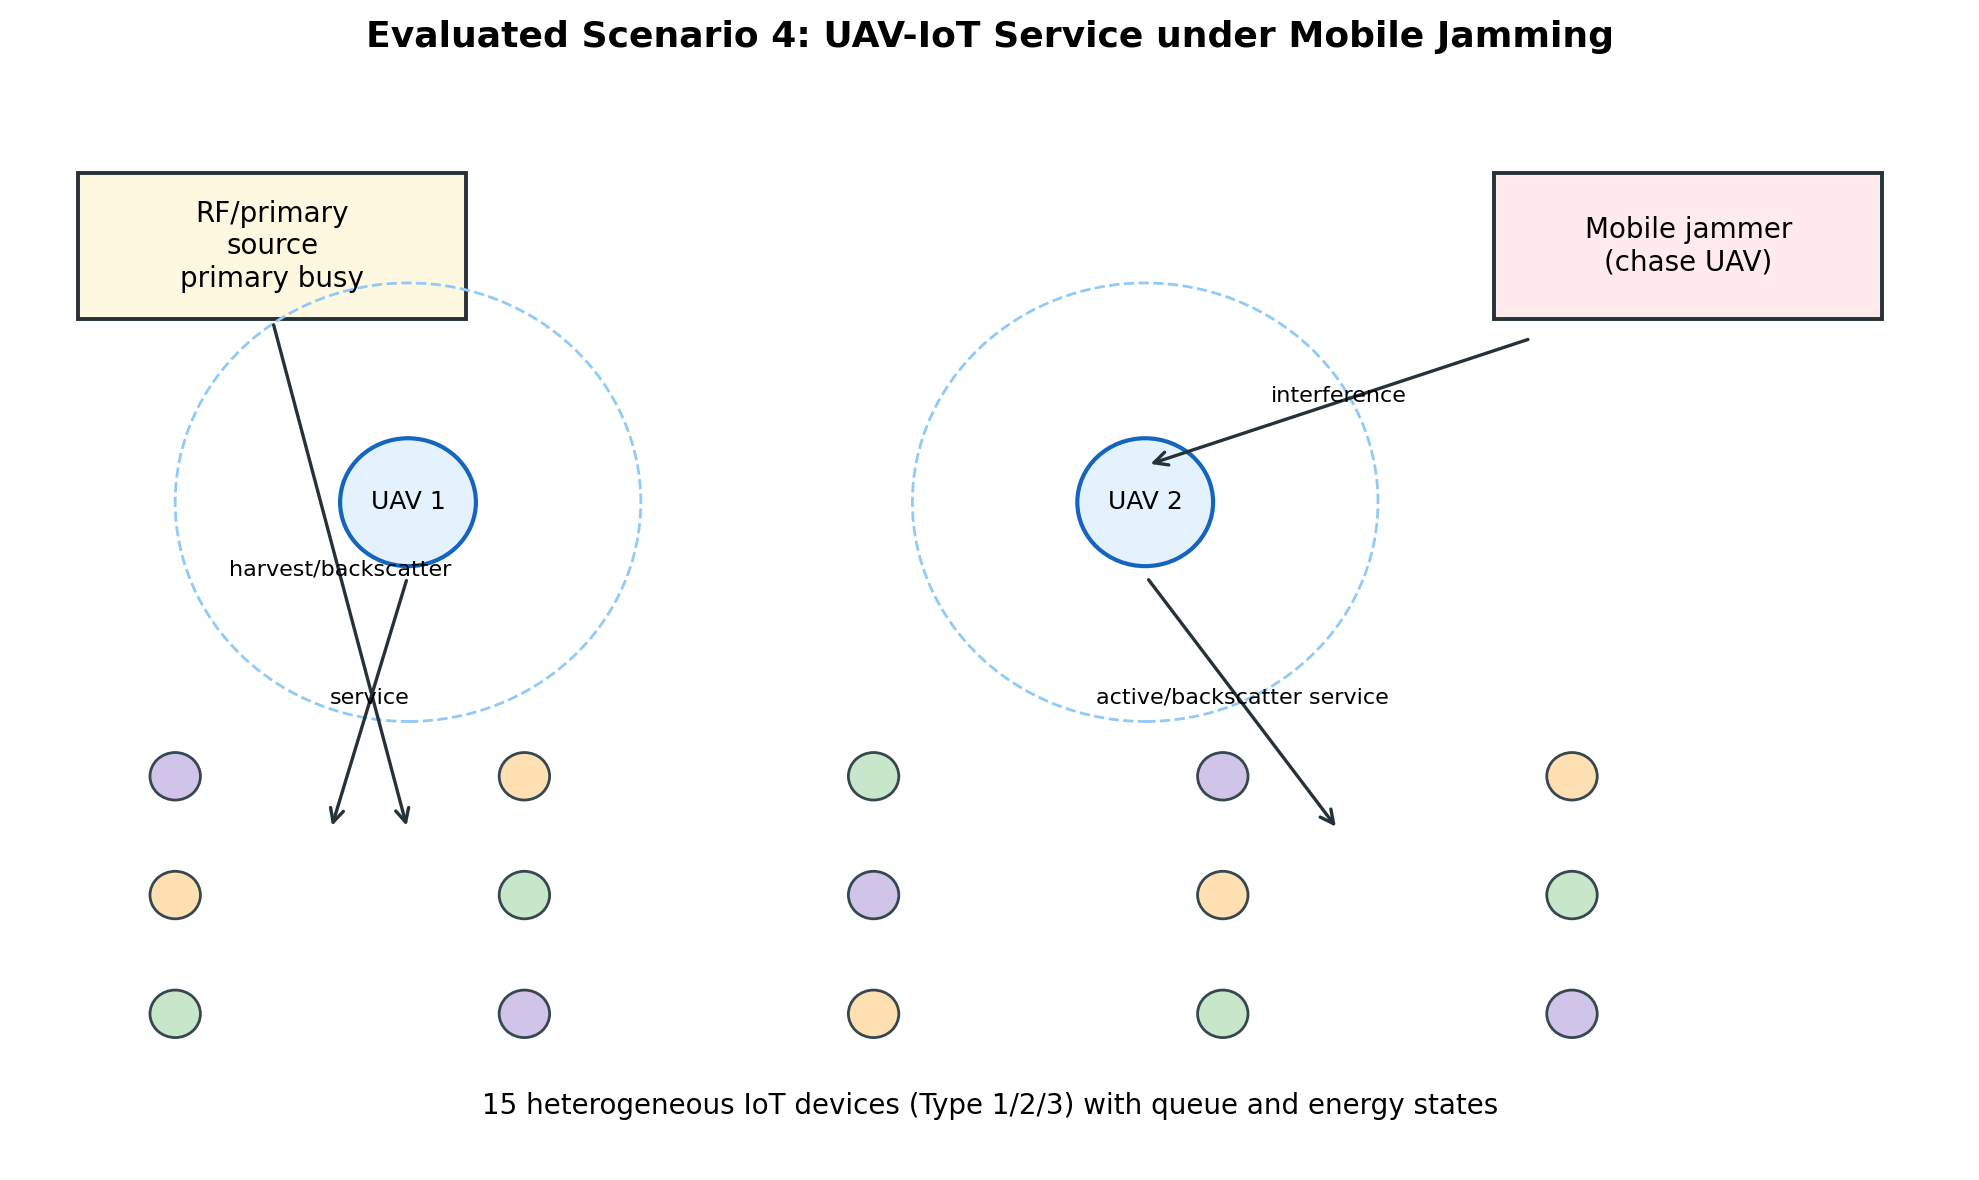
\includegraphics[width=0.92\textwidth]{system_architecture.png}
\caption{Mô hình Scenario 4: hai UAV phục vụ mười lăm thiết bị IoT dị thể dưới tác động của một jammer di động. Backscatter được mô tả ở mức trừu tượng hệ thống thông qua trạng thái primary busy và hệ số công suất hiệu dụng.}
\label{fig:system_architecture}
\end{figure}

Tại mỗi frame, IoT sinh gói, jammer di chuyển, UAV chọn hành động, môi trường cập nhật truyền thông/năng lượng/hàng đợi và trả về phần thưởng chung. Bảng \ref{tab:notation_compact} tóm tắt các ký hiệu chính.

\begin{table}[H]
\centering
\caption{Ký hiệu chính trong mô hình hệ thống.}
\label{tab:notation_compact}
\small
\begin{tabularx}{\textwidth}{lXl}
\toprule
Ký hiệu & Ý nghĩa & Giá trị trong Scenario 4 \\
\midrule
\(\mathcal{U},U\) & Tập UAV và số UAV & \(U=2\) \\
\(\mathcal{I},N\) & Tập IoT và số thiết bị IoT & \(N=15\) \\
\(\mathcal{J},J\) & Tập jammer và số jammer & \(J=1\) \\
\(L,T\) & Độ dài frame và episode & \(L=10,T=200\) \\
\(q_{i,t},B_{i,t}\) & Hàng đợi và năng lượng IoT \(i\) & Theo trạng thái mô phỏng \\
\(b_t\) & Trạng thái primary busy & Bernoulli theo cấu hình \\
\(o^u_t,s_t\) & Quan sát cục bộ và trạng thái toàn cục & \(d_o=97,d_s=70\) \\
\(a^u_t,z^u_t\) & Hành động nguyên thủy và hành động mức cao & 864 và 10 hành động \\
\bottomrule
\end{tabularx}
\end{table}

\section{Mô hình di chuyển và hàng đợi}

UAV \(u\) có vị trí \((x^u_t,y^u_t)\), độ cao cố định \(h^u\), năng lượng \(E^u_t\) và bán kính phủ \(R_{\mathrm{cov}}\). Lệnh di chuyển thuộc chín hướng rời rạc. Cập nhật vị trí có dạng:

\begin{equation}
x^u_{t+1}=\mathrm{clip}(x^u_t+\Delta_x v_{\max},0,W),\quad
y^u_{t+1}=\mathrm{clip}(y^u_t+\Delta_y v_{\max},0,H).
\label{eq:uav_mobility}
\end{equation}

% TODO: verify exact implementation form
Trong triển khai, hướng chéo được chuẩn hóa khi cập nhật vị trí; chi phí năng lượng di chuyển được tính từ chuẩn hướng rời rạc.

Mỗi IoT \(i\) có hàng đợi \(q_{i,t}\), dung lượng hàng đợi \(Q_i^{\max}\), năng lượng \(B_{i,t}\) và loại thiết bị \(c_i\in\{1,2,3\}\). Số gói đến trong frame:

\begin{equation}
A_{i,t}\sim\mathrm{Binomial}(L,p_i^{\mathrm{arr}}).
\label{eq:arrival}
\end{equation}

Cập nhật hàng đợi ở mức báo cáo:

\begin{equation}
q_{i,t+1}=\min\!\left(Q_i^{\max},q_{i,t}-D_{i,t}+A_{i,t}\right),
\label{eq:queue_update}
\end{equation}

trong đó \(D_{i,t}\) là số gói được phục vụ thành công. Gói vượt dung lượng được tính vào drop rate.

\section{Mô hình kênh và gây nhiễu}

Suy hao đường truyền:

\begin{equation}
L(d)=\max(d,1)^{\alpha},
\label{eq:path_loss}
\end{equation}

và công suất nhận:

\begin{equation}
P_{\mathrm{rx}}(P,d)=\frac{P}{L(d)}.
\label{eq:received_power}
\end{equation}

Nhiễu từ jammer \(j\) tại bộ thu \(r\):

\begin{equation}
I_{j,r}=
\begin{cases}
\dfrac{P_j}{\max(d_{j,r},1)^{\alpha}}, & d^{2D}_{j,r}\le R_j,\\
0, & \text{ngược lại}.
\end{cases}
\label{eq:jammer_interference}
\end{equation}

SINR của liên kết:

\begin{equation}
\Gamma_{a,r,t}=
\frac{P_{\mathrm{rx}}(P_a,d_{a,r})}
{N_0+\sum_{j\in\mathcal{J}}I_{j,r}}.
\label{eq:sinr}
\end{equation}

Xác suất truyền thành công được mô phỏng như:

\begin{equation}
p_{\mathrm{succ}}(\Gamma)=
\begin{cases}
1, & \theta=0,\Gamma>0,\\
0, & \theta=0,\Gamma=0,\\
\min\left(1,\dfrac{\Gamma}{\Gamma+\theta}\right), & \Gamma\ge\theta,\\
0.1\dfrac{\Gamma}{\theta}, & 0\le\Gamma<\theta.
\end{cases}
\label{eq:success_probability}
\end{equation}

Một thất bại được xem là liên quan đến gây nhiễu khi SINR thấp hơn ngưỡng và nhiễu jammer lớn hơn nhiễu nền.

\section{Năng lượng và truyền thông backscatter-inspired}

Môi trường hỗ trợ idle, harvest, backscatter, active, relay và avoid-jammer. Báo cáo tập trung vào idle/harvest/backscatter/active/avoid-jammer. Harvest tăng năng lượng IoT:

\begin{equation}
B_{i,t+1}=\min(B_i^{\max},B_{i,t}+h_i).
\label{eq:harvest_energy}
\end{equation}

Active transmission yêu cầu:

\begin{equation}
B_{i,t}\ge c_i^{\mathrm{act}},
\label{eq:active_constraint}
\end{equation}

và làm giảm năng lượng:

\begin{equation}
B_{i,t+1}=B_{i,t}-c_i^{\mathrm{act}}.
\label{eq:active_energy}
\end{equation}

Backscatter được mô phỏng bằng công suất phát hiệu dụng phụ thuộc nguồn RF và hệ số backscatter của thiết bị. Đây là abstraction ở mức hệ thống; chưa xác thực đầy đủ đặc tính vật lý ambient backscatter.

\section{Trạng thái, hành động và phần thưởng}

Quan sát cục bộ của UAV gồm trạng thái UAV, jammer gần nhất, primary busy và đặc trưng tương đối của từng IoT. Kích thước trong Scenario 4:

\begin{equation}
d_o=7+6N=97.
\label{eq:local_obs_dim}
\end{equation}

Trạng thái toàn cục:

\begin{equation}
d_s=3U+4N+2J+2=70.
\label{eq:global_state_dim}
\end{equation}

Không gian hành động phẳng và phân cấp:

\begin{equation}
|\mathcal{A}_{\mathrm{flat}}|=9(N+1)6=864,\quad
|\mathcal{A}_{\mathrm{hier}}|=10.
\label{eq:action_dims}
\end{equation}

Phần thưởng chung của môi trường:

\begin{equation}
\begin{aligned}
r_t ={}& w_{\mathrm{thr}}S_t + w_{\mathrm{avoid}}A_t
- w_{\mathrm{drop}}D_t - w_{\mathrm{delay}}\bar{q}_t \\
&- w_{\mathrm{uavE}}E^u_t - w_{\mathrm{jam}}J_t
- w_{\mathrm{col}}C_t - w_{\mathrm{unfair}}(1-F_t).
\end{aligned}
\label{eq:reward}
\end{equation}

Trong đó \(S_t\) là số gói thành công, \(A_t\) là bonus tránh jammer, \(D_t\) là số gói rơi, \(\bar{q}_t\) là hàng đợi trung bình, \(E^u_t\) là năng lượng UAV sử dụng, \(J_t\) là thất bại do nhiễu, \(C_t\) là va chạm và \(F_t\) là Jain fairness.

\section{Mục tiêu tối ưu và chỉ số đánh giá}

Mục tiêu RL ở mức báo cáo:

\begin{equation}
\max_{\pi}\mathbb{E}_{\pi}\left[\sum_{t=0}^{T-1}\gamma^t r_t\right].
\label{eq:rl_objective}
\end{equation}

% TODO: verify exact implementation form
Phương trình \eqref{eq:rl_objective} là dạng tổng quát của mục tiêu học; cập nhật cụ thể phụ thuộc DDQN hoặc QMIX.

Các chỉ số đánh giá chính:

\begin{align}
\eta &= \frac{\sum_i D_i}{T_{\mathrm{ep}}}, \label{eq:throughput}\\
\rho_{\mathrm{drop}} &= \frac{\sum_i \mathrm{Dropped}_i}{\max(\sum_i \mathrm{Arrived}_i,1)}, \label{eq:drop_rate}\\
\rho_{\mathrm{jam}} &= \frac{\mathrm{jamming\ failures}}{\max(\mathrm{transmission\ attempts},1)}, \label{eq:jam_rate}\\
F &= \frac{(\sum_i D_i)^2}{N\sum_iD_i^2+\epsilon}, \label{eq:jain}\\
\xi &= \frac{\sum_iD_i}{\max(E_{\mathrm{UAV}}+E_{\mathrm{IoT}},10^{-9})}. \label{eq:energy_efficiency}
\end{align}

Bài toán cuối cùng là học chính sách UAV hợp tác nhằm tăng thông lượng và giảm rơi gói/gây nhiễu, đồng thời duy trì công bằng và hiệu quả năng lượng trong phạm vi mô phỏng đã triển khai.

\chapter{Phương pháp đề xuất}

\section{Tổng quan pipeline}

Phương pháp được xây dựng theo ba bước. Thứ nhất, Flat DDQN được dùng như baseline học trực tiếp trên hành động nguyên thủy. Thứ hai, Hierarchical DDQN kiểm tra tác dụng của giao diện hành động mức cao. Thứ ba, QMIX-Hierarchical dùng cùng giao diện 10 hành động để học phối hợp nhiều UAV.

Trọng tâm của phương pháp là giảm độ khó học bằng action abstraction. Trong Scenario 4, hành động nguyên thủy có 864 tổ hợp, còn hành động phân cấp chỉ có 10 lựa chọn mức cao. Hình \ref{fig:hier_action_arch} tóm tắt pipeline này.

\begin{figure}[H]
\centering
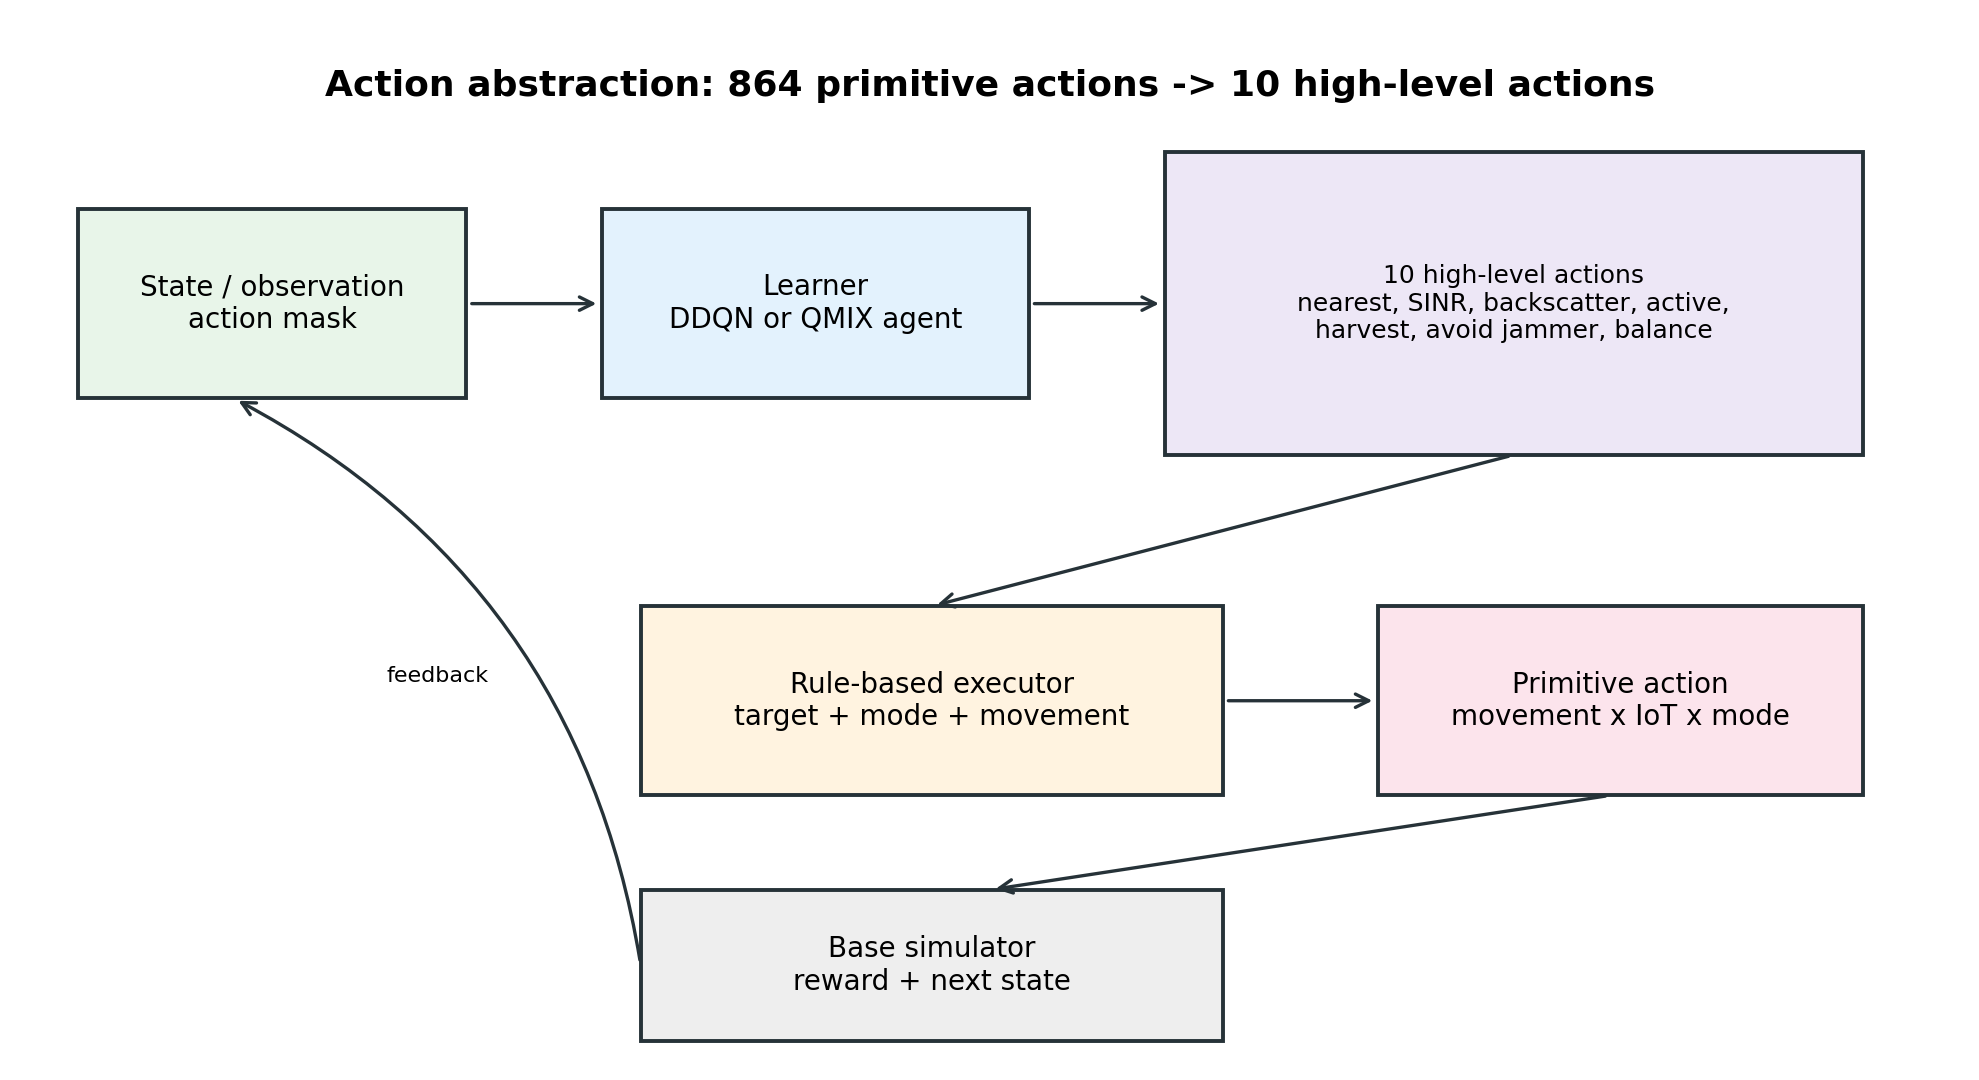
\includegraphics[width=0.94\textwidth]{hierarchical_action_architecture.png}
\caption{Giao diện hành động phân cấp. Tác tử học chọn một trong 10 hành động mức cao; executor dựa trên quy tắc chuyển hành động này thành bộ ba nguyên thủy gồm di chuyển, IoT mục tiêu và chế độ truyền thông.}
\label{fig:hier_action_arch}
\end{figure}

\section{Flat DDQN baseline}

Hành động phẳng của UAV \(u\) là:

\begin{equation}
a^u_t=(m^u_t,i^u_t,c^u_t),
\label{eq:flat_action}
\end{equation}

trong đó \(m^u_t\) là lệnh di chuyển, \(i^u_t\) là IoT mục tiêu và \(c^u_t\) là chế độ truyền thông. Với 15 IoT, số hành động là 864. DDQN dùng mục tiêu Double-DQN:

\begin{equation}
y_t=r_t+\gamma(1-d_t)Q^{-}\!\left(s_{t+1},
\arg\max_{a'}Q(s_{t+1},a')\right).
\label{eq:ddqn_target}
\end{equation}

Flat DDQN giữ nguyên ngữ nghĩa hành động của mô phỏng nên là baseline cần thiết. Tuy nhiên, nhiều hành động phẳng không hợp lệ hoặc ít giá trị trong từng trạng thái, làm việc học kém hiệu quả.

\section{Trừu tượng hóa hành động phân cấp}

Thay vì chọn \(a^u_t\), UAV chọn hành động mức cao:

\begin{equation}
z^u_t\in\mathcal{Z},\quad |\mathcal{Z}|=10.
\label{eq:high_action}
\end{equation}

Bảng \ref{tab:high_level_actions} liệt kê mười hành động mức cao được dùng trong executor.

\begin{table}[H]
\centering
\caption{Mười hành động mức cao trong executor phân cấp.}
\label{tab:high_level_actions}
\small
\begin{tabularx}{\textwidth}{clX}
\toprule
ID & Hành động & Hành vi chính \\
\midrule
0 & IDLE\_SAFE & Nghỉ hoặc chỉ truyền khi cơ hội đủ an toàn. \\
1 & SERVE\_NEAREST\_QUEUE & Phục vụ IoT gần nhất có hàng đợi. \\
2 & SERVE\_BEST\_SINR & Ưu tiên IoT có SINR tốt. \\
3 & PRIORITIZE\_BACKSCATTER\_TYPE23 & Ưu tiên Type 2/3 và backscatter. \\
4 & PRIORITIZE\_ACTIVE\_TYPE1 & Ưu tiên Type 1 và active. \\
5 & HARVEST\_LOW\_ENERGY & Hỗ trợ thiết bị năng lượng thấp và harvest. \\
6 & AVOID\_JAMMER & Tránh jammer và giảm rủi ro nhiễu. \\
7 & BALANCE\_UNDERSERVED\_IOT & Ưu tiên thiết bị được phục vụ ít. \\
8 & HYBRID\_BALANCED & Kết hợp hàng đợi, SINR, loại thiết bị, fairness và jammer risk. \\
9 & HIGH\_QUEUE\_PRIORITY & Ưu tiên áp lực hàng đợi cao. \\
\bottomrule
\end{tabularx}
\end{table}

Executor thực hiện ánh xạ:

\begin{equation}
\phi_{\mathrm{exec}}:(\mathbf{z}_t,s_t)\mapsto \mathbf{a}_t.
\label{eq:executor_mapping}
\end{equation}

Executor là rule-based, không phải mạng học. Nó dùng thông tin môi trường như vị trí UAV/IoT, hàng đợi, năng lượng, loại thiết bị, primary busy, jammer và điểm SINR để chọn hành động nguyên thủy. Đây là ưu điểm về tri thức miền nhưng cũng là một giới hạn cần nêu rõ.

\section{Hierarchical DDQN}

Hierarchical DDQN giữ cấu trúc DDQN nhưng đầu ra là \(z^u_t\in\mathcal{Z}\). Trạng thái đầu vào là kết hợp giữa global state và local observation. Action mask được áp dụng trước epsilon-greedy để tránh chọn hành động mức cao không hợp lệ hoặc bị vô hiệu hóa. Phương pháp này được dùng để kiểm tra giả thuyết: nút thắt chính của Flat DDQN là giao diện hành động, không chỉ là kiến trúc mạng.

\section{QMIX-Hierarchical}

QMIX-Hierarchical là phương pháp MaDRL chính. Mỗi UAV là một tác tử, nhận quan sát cục bộ \(o^u_t\) và chọn hành động mức cao \(z^u_t\). Mạng agent chia sẻ tham số ước lượng:

\begin{equation}
Q_u(o^u_t,z^u_t;\theta).
\label{eq:agent_q}
\end{equation}

Mixer nhận các giá trị agent đã chọn và trạng thái toàn cục:

\begin{equation}
Q_{\mathrm{tot}}(s_t,\mathbf{z}_t)
=f_{\mathrm{mix}}(Q_1,\ldots,Q_U,s_t;\psi).
\label{eq:qmix_mixer}
\end{equation}

QMIX áp đặt ràng buộc đơn điệu:

\begin{equation}
\frac{\partial Q_{\mathrm{tot}}}{\partial Q_u}\ge 0,\quad \forall u.
\label{eq:qmix_monotonic}
\end{equation}

Hình \ref{fig:qmix_arch} mô tả cấu trúc huấn luyện và thực thi.

\begin{figure}[H]
\centering
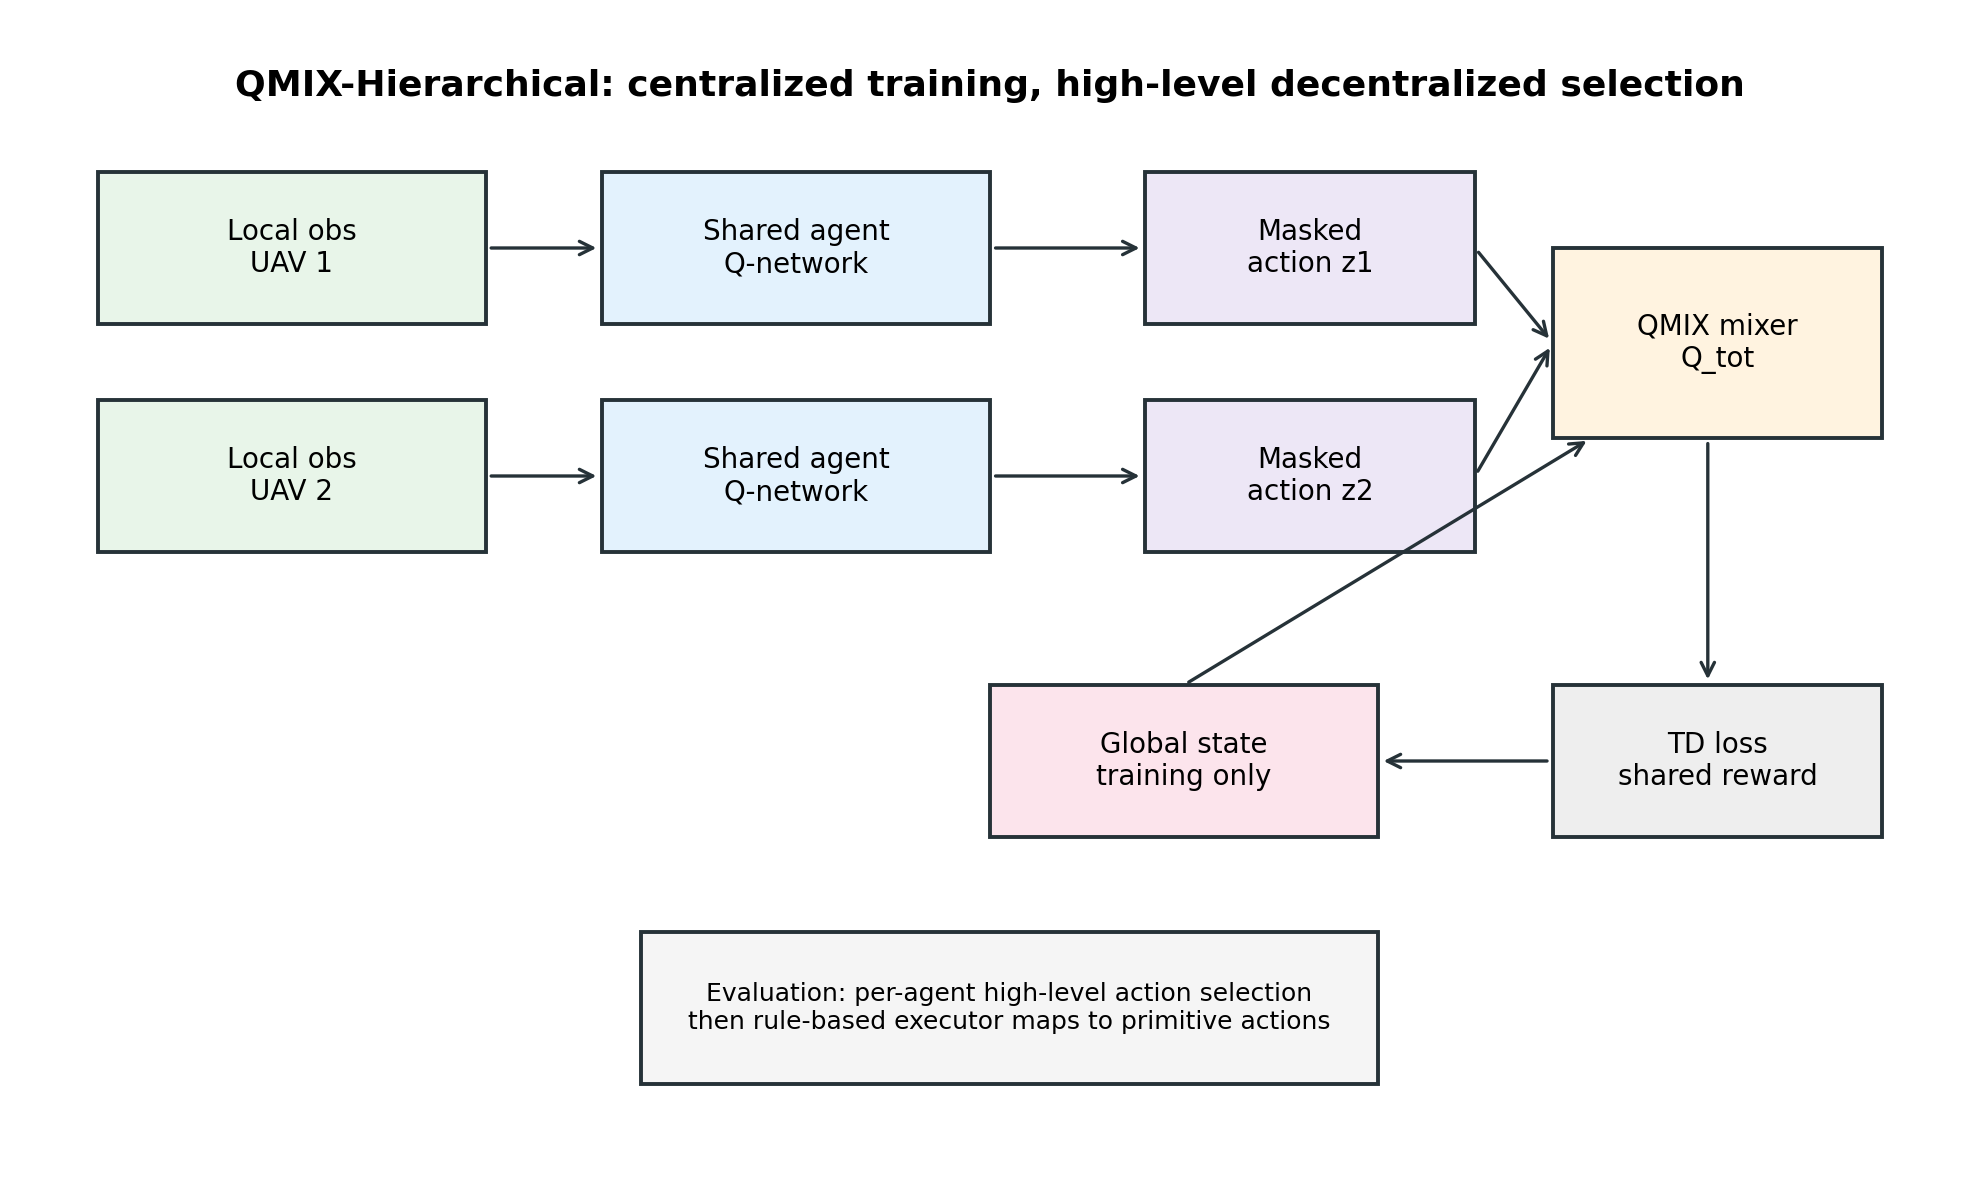
\includegraphics[width=0.95\textwidth]{qmix_architecture.png}
\caption{QMIX-Hierarchical. Trong huấn luyện, mixer sử dụng trạng thái toàn cục và phần thưởng chung để học \(Q_{\mathrm{tot}}\). Trong đánh giá, mỗi UAV chọn hành động mức cao từ quan sát cục bộ, sau đó executor chuyển sang hành động nguyên thủy.}
\label{fig:qmix_arch}
\end{figure}

\section{Huấn luyện và thực thi}

QMIX được huấn luyện tập trung: replay buffer lưu trajectory chung, mixer dùng global state, và phần thưởng là phần thưởng mạng. Chọn hành động mức cao mang tính cục bộ: mỗi UAV dùng quan sát của mình và agent id để tính Q-value trên 10 hành động.

Điểm cần nhấn mạnh là quá trình thực thi nguyên thủy không hoàn toàn phi tập trung, vì executor vẫn dùng thông tin môi trường để ánh xạ hành động mức cao. Do đó, báo cáo dùng cách diễn đạt: decentralized high-level action selection with a rule-based executor.

Mục tiêu TD của QMIX:

\begin{equation}
y_t=r_t+\gamma(1-d_t)Q_{\mathrm{tot}}^{-}(s_{t+1},\mathbf{z}^{*}_{t+1}),
\label{eq:qmix_target}
\end{equation}

và hàm mất mát:

\begin{equation}
\mathcal{L}=
\frac{\sum_{b,t}M_{b,t}\left(Q_{\mathrm{tot}}(s_{b,t},\mathbf{z}_{b,t})-y_{b,t}\right)^2}
{\sum_{b,t}M_{b,t}}.
\label{eq:qmix_loss}
\end{equation}

\section{Pseudocode tóm tắt}

\begin{algorithm}[H]
\caption{Huấn luyện QMIX-Hierarchical}
\label{alg:qmix_short}
\begin{algorithmic}[1]
\State Khởi tạo môi trường, wrapper phân cấp, agent network và mixer.
\For{mỗi episode}
  \State Reset môi trường, tạo trajectory rỗng.
  \For{mỗi frame}
    \For{mỗi UAV \(u\)}
      \State Tính \(Q_u(o^u_t,\cdot)\), áp dụng action mask và chọn \(z^u_t\).
    \EndFor
    \State Executor ánh xạ \(\mathbf{z}_t\) thành \(\mathbf{a}_t\); môi trường trả về \(r_t\).
    \State Lưu observation, state, action, reward, mask và next state vào trajectory.
  \EndFor
  \State Cập nhật agent network và mixer bằng \eqref{eq:qmix_loss} nếu replay đủ lớn.
\EndFor
\end{algorithmic}
\end{algorithm}

\section{Tóm tắt phương pháp}

Flat DDQN kiểm tra giới hạn của điều khiển nguyên thủy. Hierarchical DDQN chứng minh rằng giảm hành động từ 864 xuống 10 làm bài toán khả học hơn. QMIX-Hierarchical là phương pháp MaDRL cuối cùng vì kết hợp action abstraction với value decomposition hợp tác giữa UAV. Các giới hạn gồm executor rule-based, backscatter abstraction và fairness chưa được giải quyết hoàn toàn.

\chapter{Thực nghiệm, kết quả và thảo luận}

\section{Thiết lập thực nghiệm}

Các kết quả trong chương này được lấy từ artifact Phase 3 đã có; không huấn luyện lại mô hình và không thay đổi tham số mô phỏng. Benchmark chính là Scenario 4: 2 UAV, 15 IoT dị thể, 1 jammer di động, frame length 10 và episode length 200. Bảng \ref{tab:scenario_metrics} tóm tắt kịch bản và chỉ số.

\begin{table}[H]
\centering
\caption{Kịch bản mô phỏng và chỉ số đánh giá.}
\label{tab:scenario_metrics}
\scriptsize
\resizebox{\textwidth}{!}{\begin{tabular}{lllllll}
\hline
Section & Scenario / Metric & UAV count & IoT count & Jammer setting & Backscatter/active relevance & Purpose \\
\hline
Scenario & No-jammer calibrated & 1 & 5 & Disabled & Basic backscatter/active scheduling without jamming. & Learnability sanity check and no-jammer reference. \\
Scenario & Static weak jammer & 2 & 10 & One weak static jammer & Anti-jamming behavior with moderate coordination. & Intermediate transfer and robustness validation. \\
Scenario & Scenario 4 backscatter types & 2 & 15 & One calibrated mobile/chase jammer & Heterogeneous Type 1/2/3 devices with active, backscatter, and harvest modes. & Main heterogeneous RF-powered backscatter coordination benchmark. \\
Metric & Throughput/frame &  &  &  &  & Delivered packets per frame; higher is better. \\
Metric & Drop rate &  &  &  &  & Fraction of generated/queued packets dropped; lower is better. \\
Metric & Jamming failure &  &  &  &  & Transmission failures attributed to jamming; lower is better. \\
Metric & Fairness &  &  &  &  & Jain-style service fairness across IoT devices; higher is better. \\
Metric & Energy efficiency &  &  &  &  & Delivered utility per energy cost; higher is better. \\
Metric & Backscatter success &  &  &  &  & Successful backscatter transmission rate; higher is better. \\
Metric & Active success &  &  &  &  & Successful active transmission rate; higher is better. \\
\hline
\end{tabular}
}
\end{table}

Các phương pháp gồm Random, HTT-only, Backscatter-only, Greedy SINR, Greedy nearest, Flat DDQN, Hierarchical DDQN, QMIX-Hierarchical và các ablation công bằng. Flat DDQN và Hierarchical DDQN là kết quả đơn chạy trong gói artifact hiện tại; QMIX base và các ablation chính được báo cáo theo ba seed.

\section{So sánh tổng thể trong Scenario 4}

Bảng \ref{tab:overall_scenario4} và Hình \ref{fig:overall_throughput} cho thấy Flat DDQN đạt throughput/frame 0.3242, gần HTT-only 0.3278 và thấp hơn đáng kể so với các phương pháp phân cấp. Điều này hỗ trợ nhận định rằng giao diện hành động nguyên thủy 864 hành động gây khó khăn cho baseline DDQN đã triển khai.

\begin{table}[H]
\centering
\caption{So sánh tổng thể trong Scenario 4. QMIX base được báo cáo theo mean/std trên ba seed; Flat DDQN và Hierarchical DDQN là kết quả đơn chạy trong artifact hiện tại.}
\label{tab:overall_scenario4}
\scriptsize
\resizebox{\textwidth}{!}{\input{../../results/publication_tables/table1_overall_scenario4_comparison.tex}}
\end{table}

\begin{figure}[H]
\centering
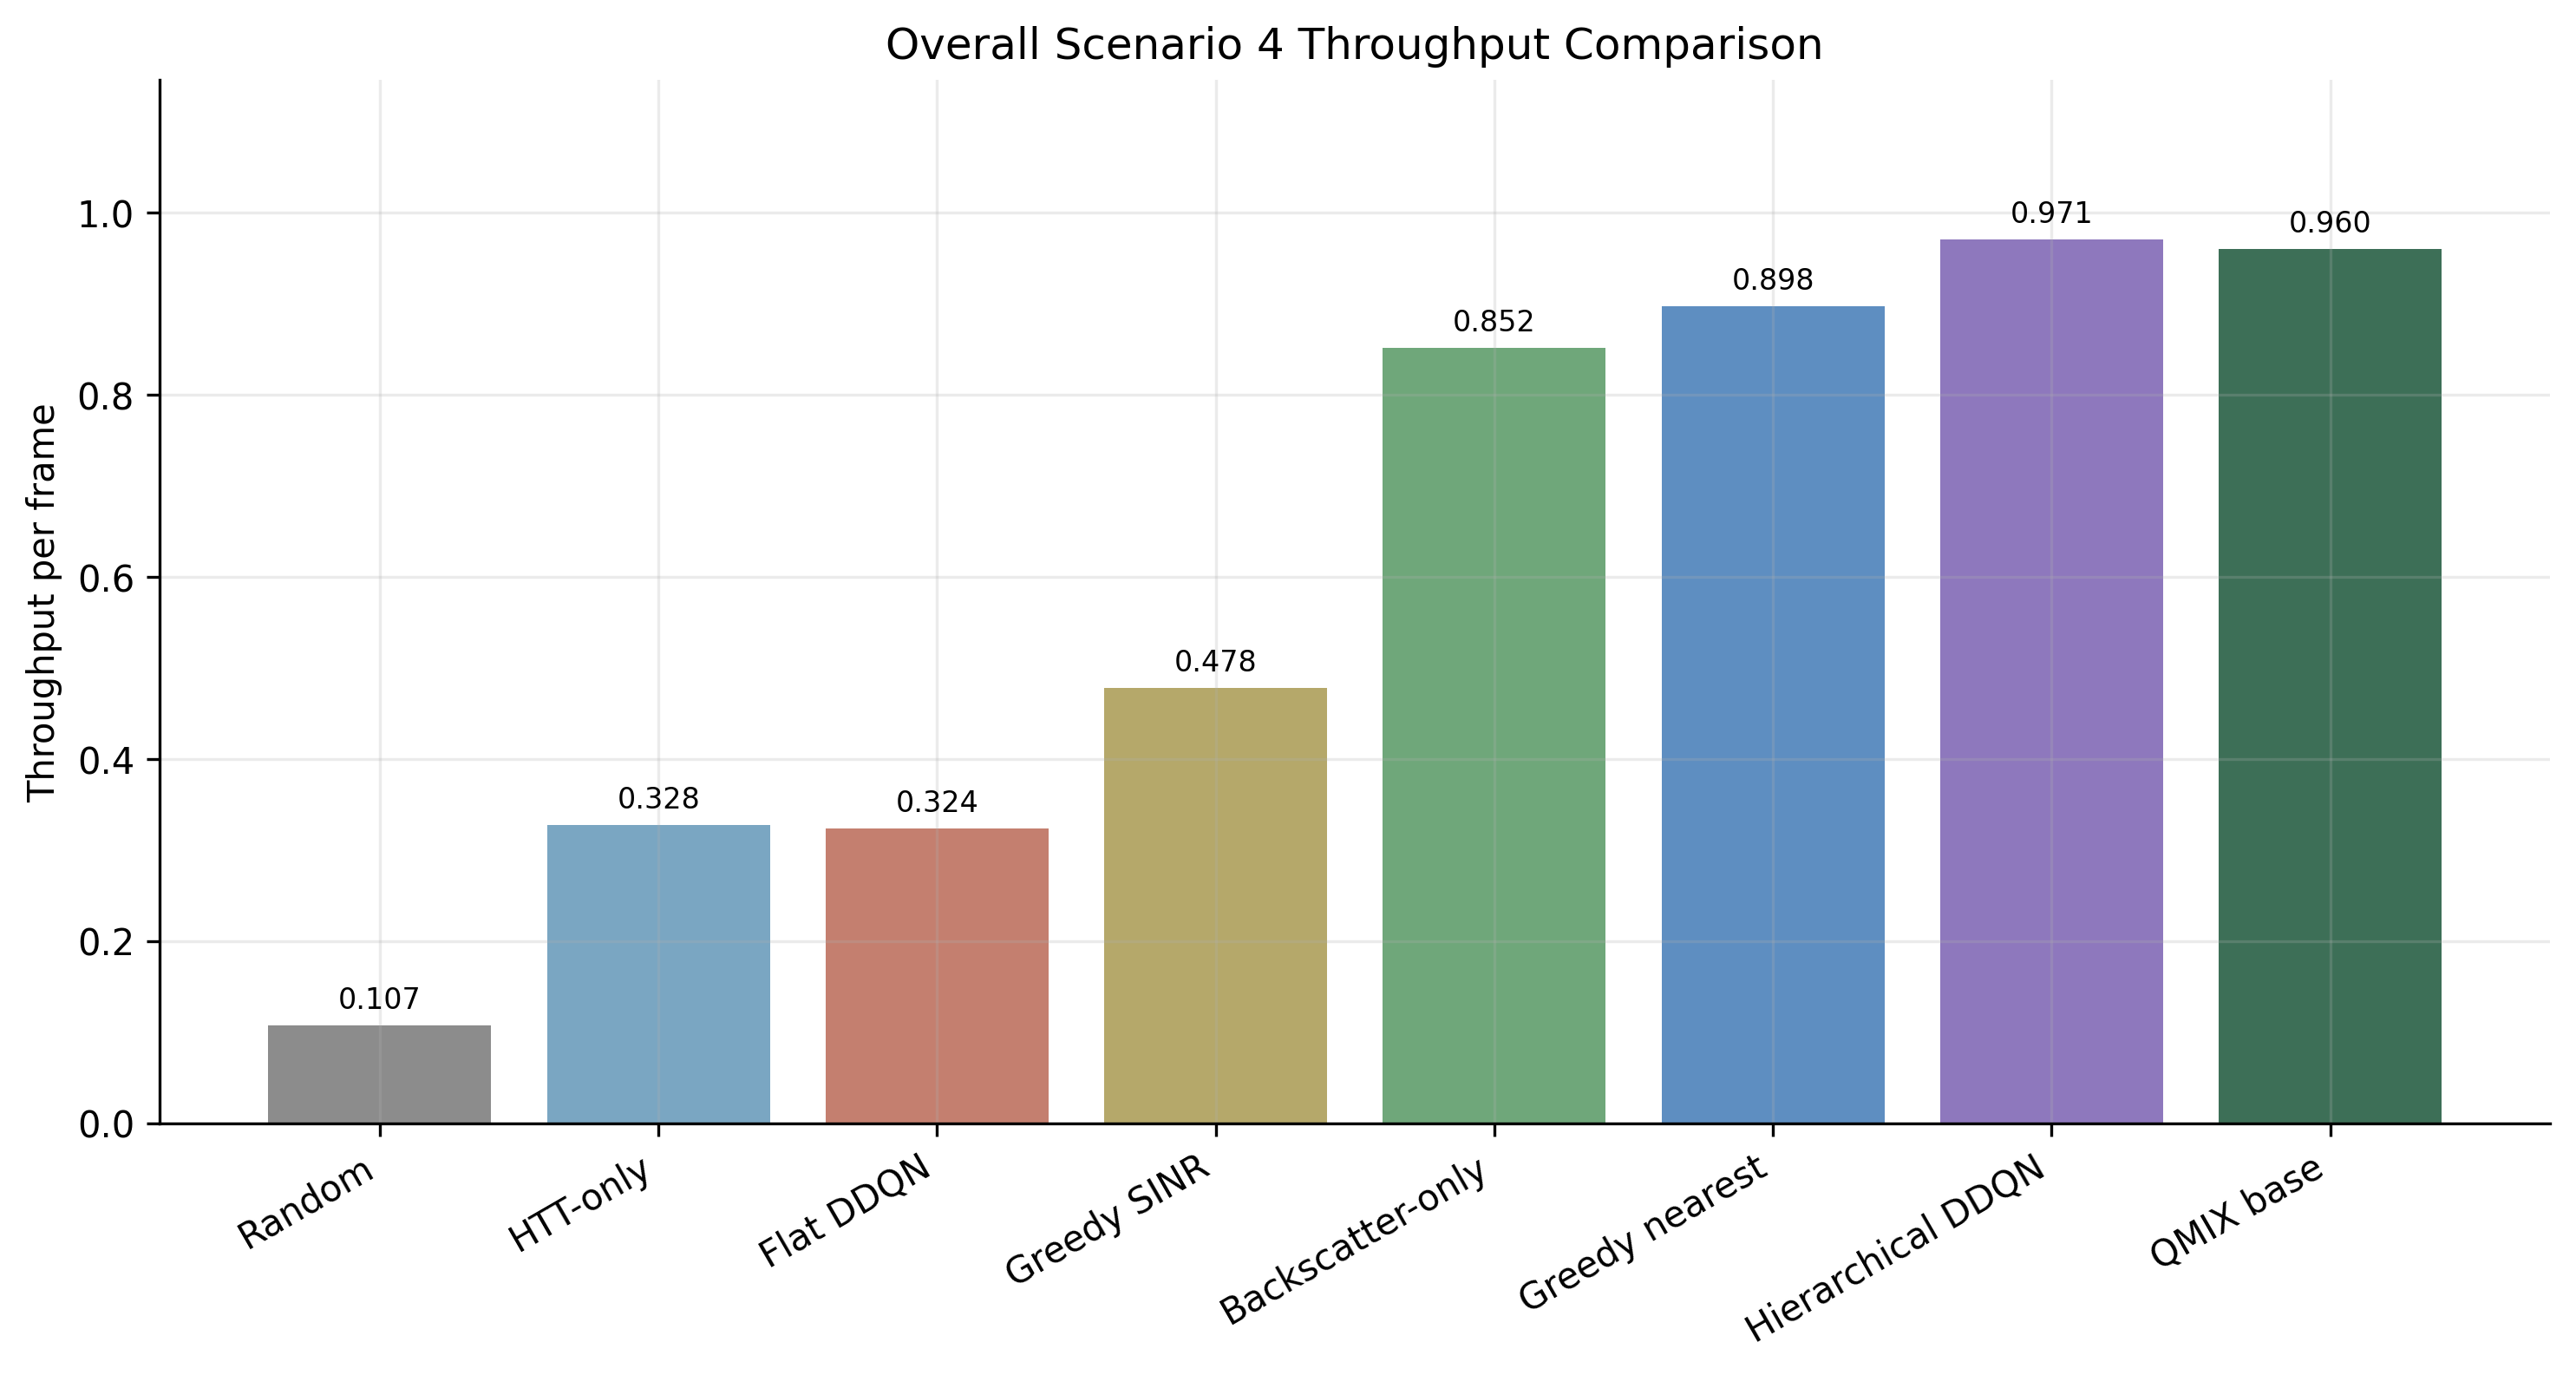
\includegraphics[width=0.9\textwidth]{fig1_overall_throughput_comparison.png}
\caption{Throughput/frame của các baseline và phương pháp học trong Scenario 4. Hình này nhấn mạnh khoảng cách giữa Flat DDQN và các phương pháp dùng hành động phân cấp.}
\label{fig:overall_throughput}
\end{figure}

Hierarchical DDQN đạt throughput/frame 0.9710, cho thấy việc giảm giao diện từ 864 xuống 10 hành động giúp bài toán khả học hơn. QMIX base đạt \(0.9604\pm0.0255\), thấp hơn nhẹ so với Hierarchical DDQN đơn chạy về throughput; vì vậy báo cáo không khẳng định QMIX vượt Hierarchical DDQN về thông lượng trung bình. Điểm mạnh của QMIX là ổn định đa seed và cải thiện các chỉ số phối hợp như jamming failure và fairness.

\begin{figure}[H]
\centering
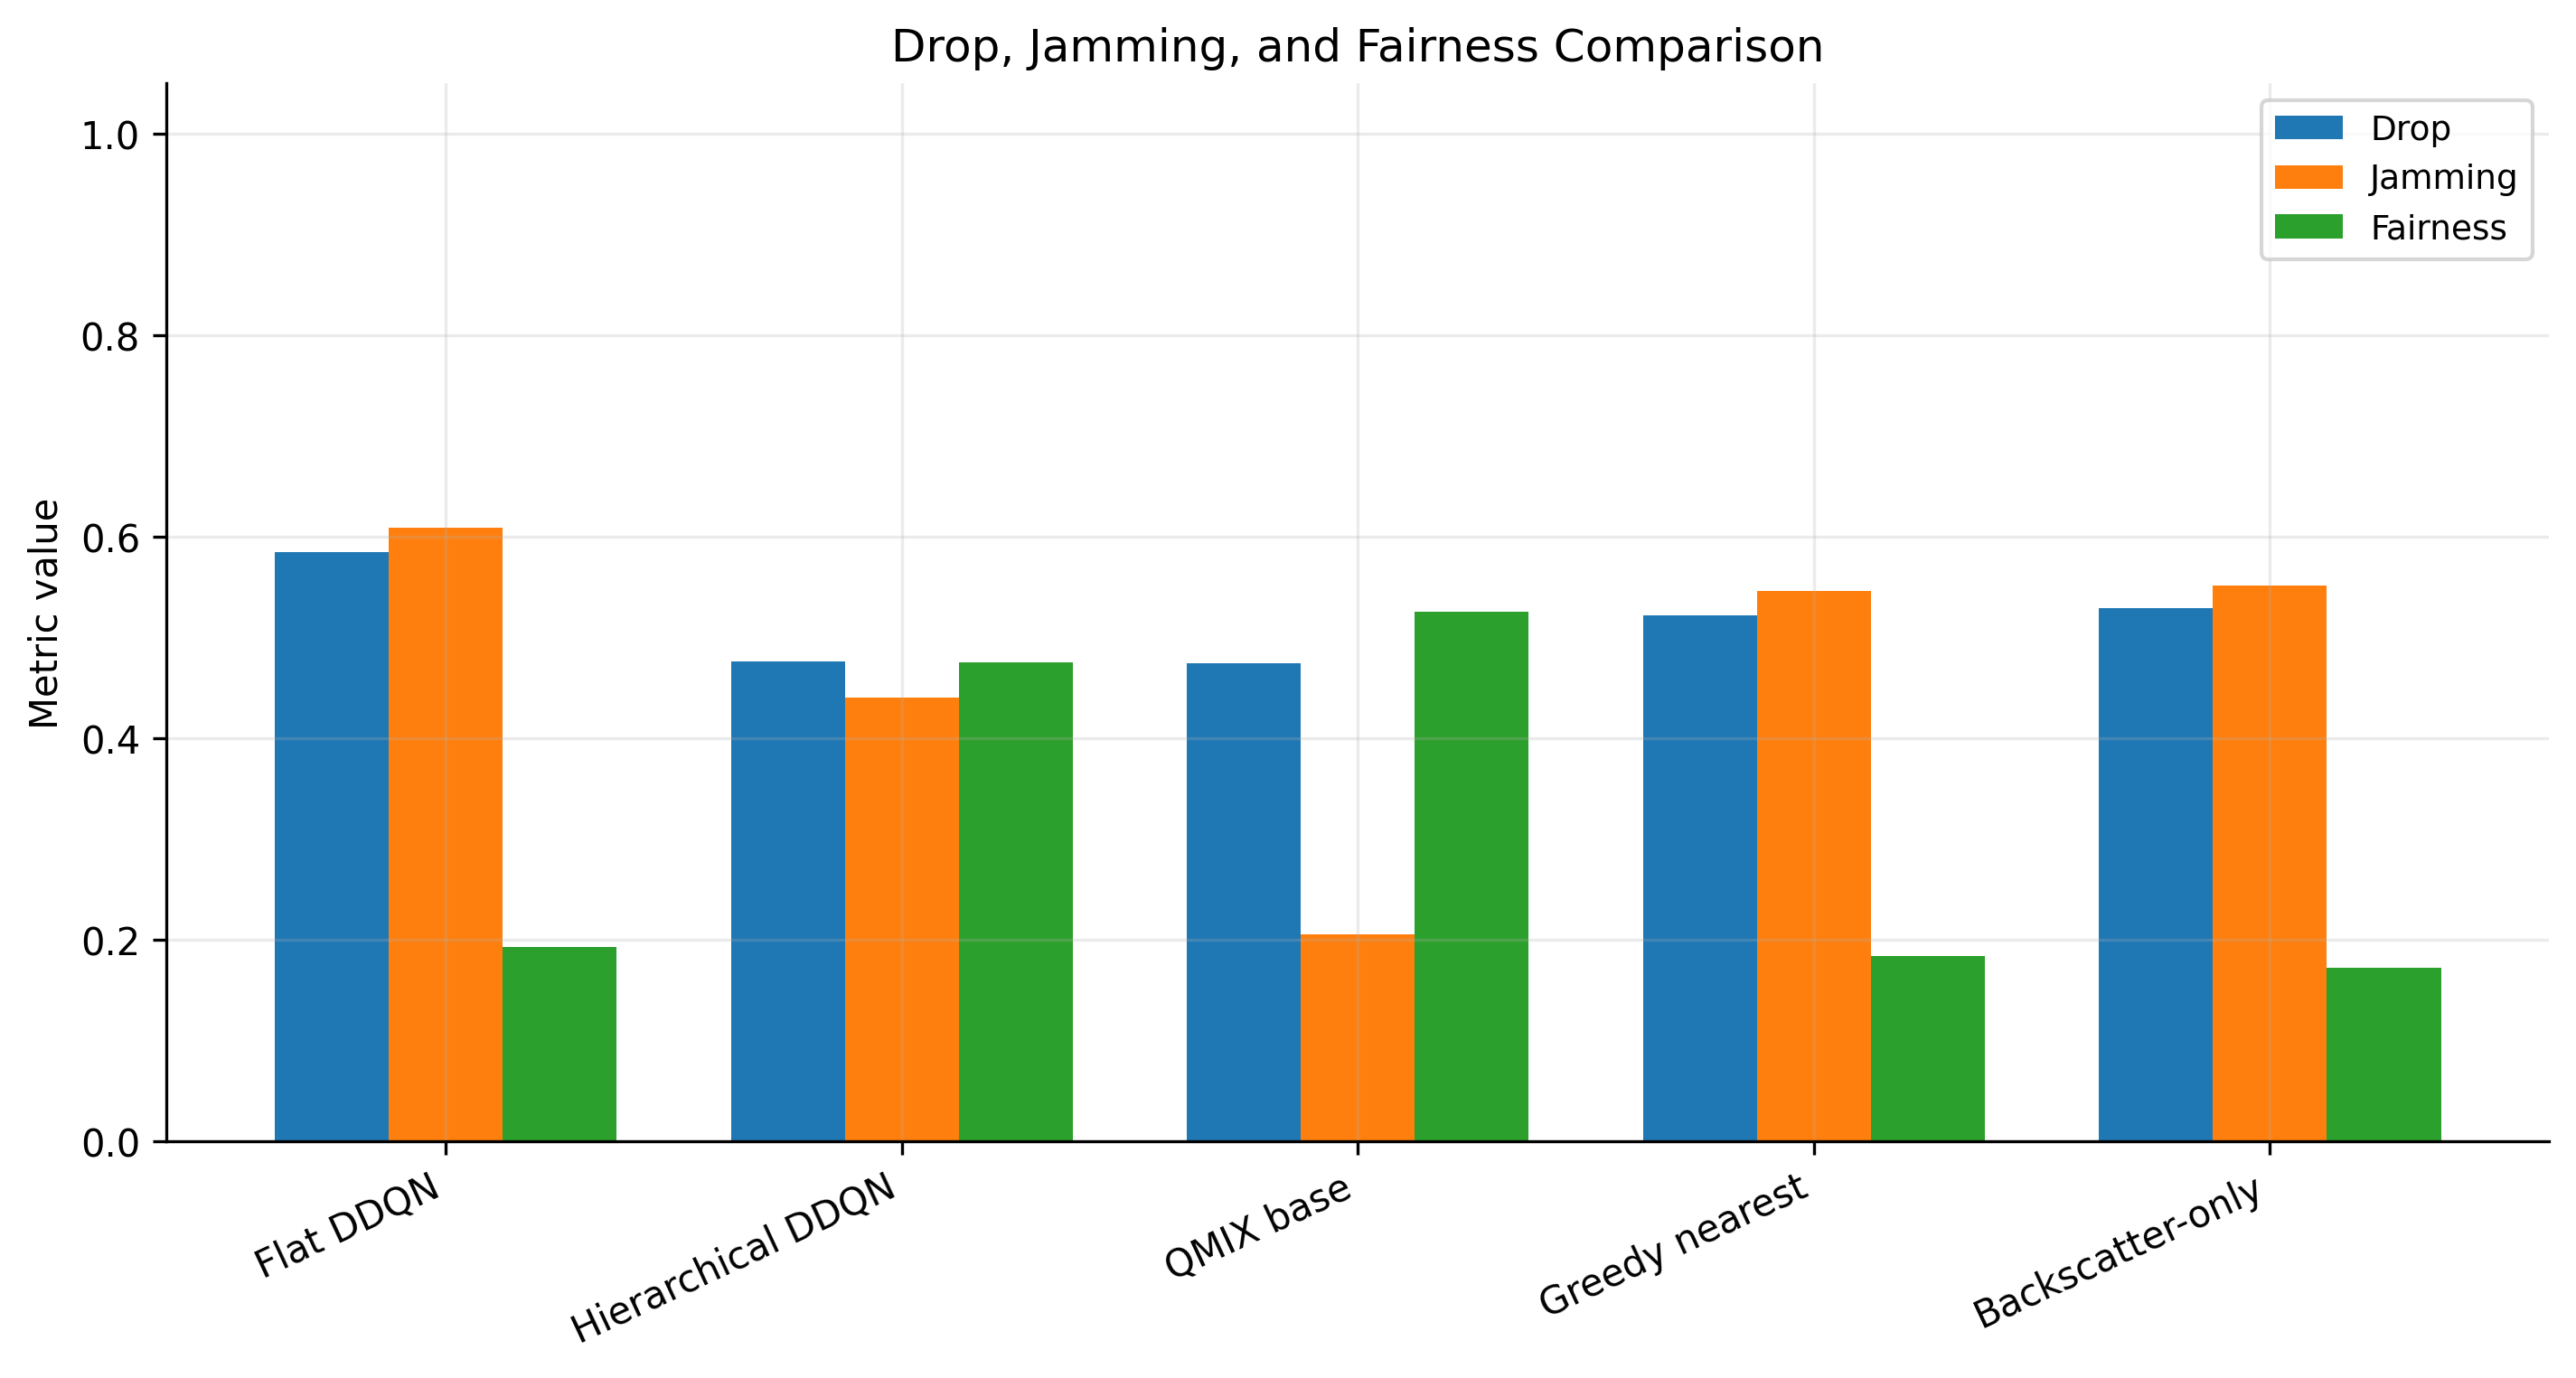
\includegraphics[width=0.9\textwidth]{fig2_drop_jam_fairness_comparison.png}
\caption{So sánh drop rate, jamming failure và fairness. QMIX base giảm jamming failure và cải thiện fairness so với Hierarchical DDQN trong gói kết quả hiện có.}
\label{fig:drop_jam_fairness}
\end{figure}

\section{Tiến trình thuật toán}

Bảng \ref{tab:algorithm_progression} và Hình \ref{fig:algorithm_progression} trình bày tiến trình từ Flat DDQN sang Hierarchical DDQN và QMIX-Hierarchical. Bước cải thiện lớn nhất là thay đổi giao diện hành động, không phải chỉ thay đổi mạng học.

\begin{table}[H]
\centering
\caption{Tiến trình thuật toán từ hành động phẳng đến hành động phân cấp và QMIX.}
\label{tab:algorithm_progression}
\scriptsize
\resizebox{\textwidth}{!}{\begin{tabular}{lllllllll}
\hline
Method & Action interface & Action dimension & Multi-agent coordination & Throughput/frame & Drop rate & Jamming failure & Fairness & Interpretation \\
\hline
Flat DDQN & Flat movement x IoT x mode & 864 & Centralized-factorized DDQN & 0.3242 & 0.5846 & 0.6093 & 0.1930 & Large flat action space limits learning in heterogeneous Scenario 4. \\
Flat DDQN + tuning & Flat movement x IoT x mode & 864 & Centralized-factorized DDQN & 0.1203 & 0.6073 & 0.5557 & 0.1374 & Reward scaling and dueling stabilized loss but did not solve the action-interface bottleneck. \\
Hierarchical DDQN & High-level executor & 10 & Centralized-factorized DDQN & 0.9710 & 0.4761 & 0.4403 & 0.4754 & Action abstraction is the dominant improvement over flat DDQN. \\
QMIX-Hierarchical & High-level executor & 10 & QMIX value decomposition & 0.9604 & 0.4744 & 0.2056 & 0.5260 & QMIX preserves high throughput and improves jamming/fairness trade-off over hierarchical DDQN. \\
\hline
\end{tabular}
}
\end{table}

\begin{figure}[H]
\centering
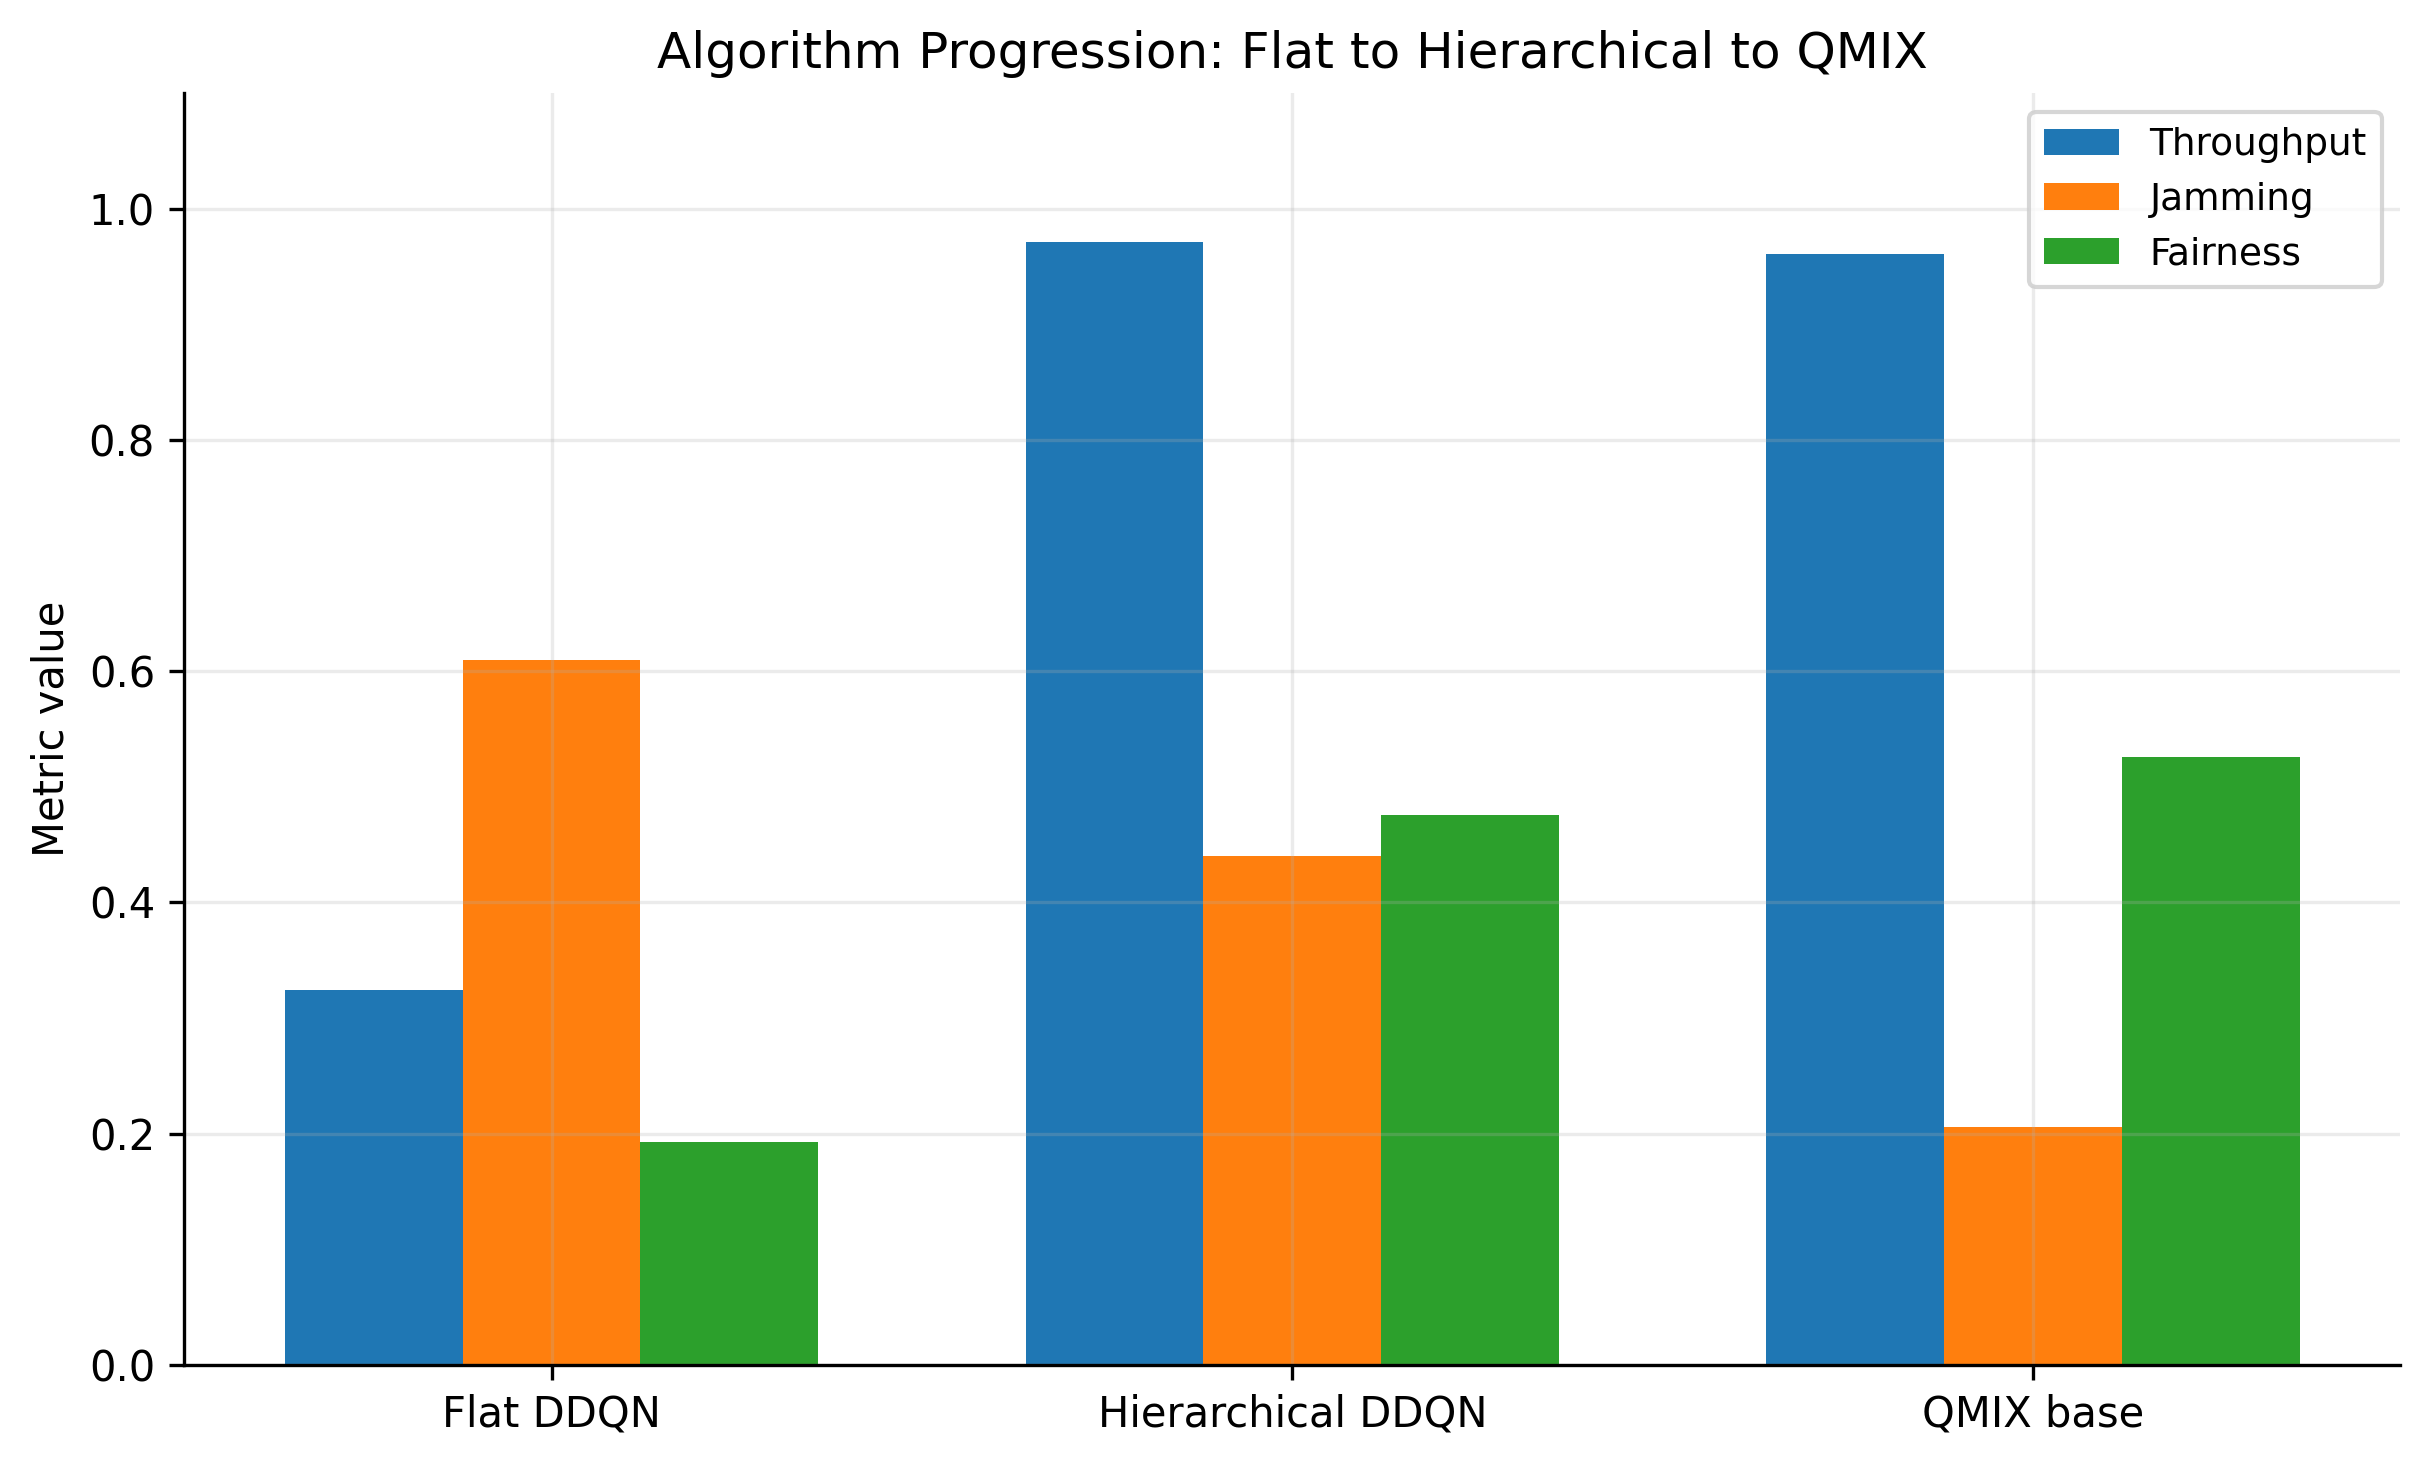
\includegraphics[width=0.84\textwidth]{fig3_algorithm_progression.png}
\caption{Tiến trình kết quả: Flat DDQN cho thấy nút thắt không gian hành động; Hierarchical DDQN chứng minh hiệu quả action abstraction; QMIX thêm phối hợp đa tác tử.}
\label{fig:algorithm_progression}
\end{figure}

Flat DDQN + tuning trong Bảng \ref{tab:algorithm_progression} chỉ là kết quả hỗ trợ: reward scaling và dueling giúp ổn định một số khía cạnh huấn luyện nhưng không giải quyết nút thắt hành động phẳng. Phương pháp cuối cùng vì vậy giữ giao diện phân cấp và chuyển sang QMIX.

\section{Ổn định đa seed của QMIX}

Bảng \ref{tab:qmix_multiseed} báo cáo QMIX base trên seed 42, 43 và 44. Kết quả trung bình đạt throughput/frame \(0.9604\pm0.0255\), drop \(0.4744\pm0.0054\), jamming failure \(0.2056\pm0.0744\) và fairness \(0.5260\pm0.0572\).

\begin{table}[H]
\centering
\caption{Kết quả QMIX base theo seed và thống kê mean/std.}
\label{tab:qmix_multiseed}
\scriptsize
\resizebox{\textwidth}{!}{\input{../../results/publication_tables/table3_qmix_multiseed.tex}}
\end{table}

\begin{figure}[H]
\centering
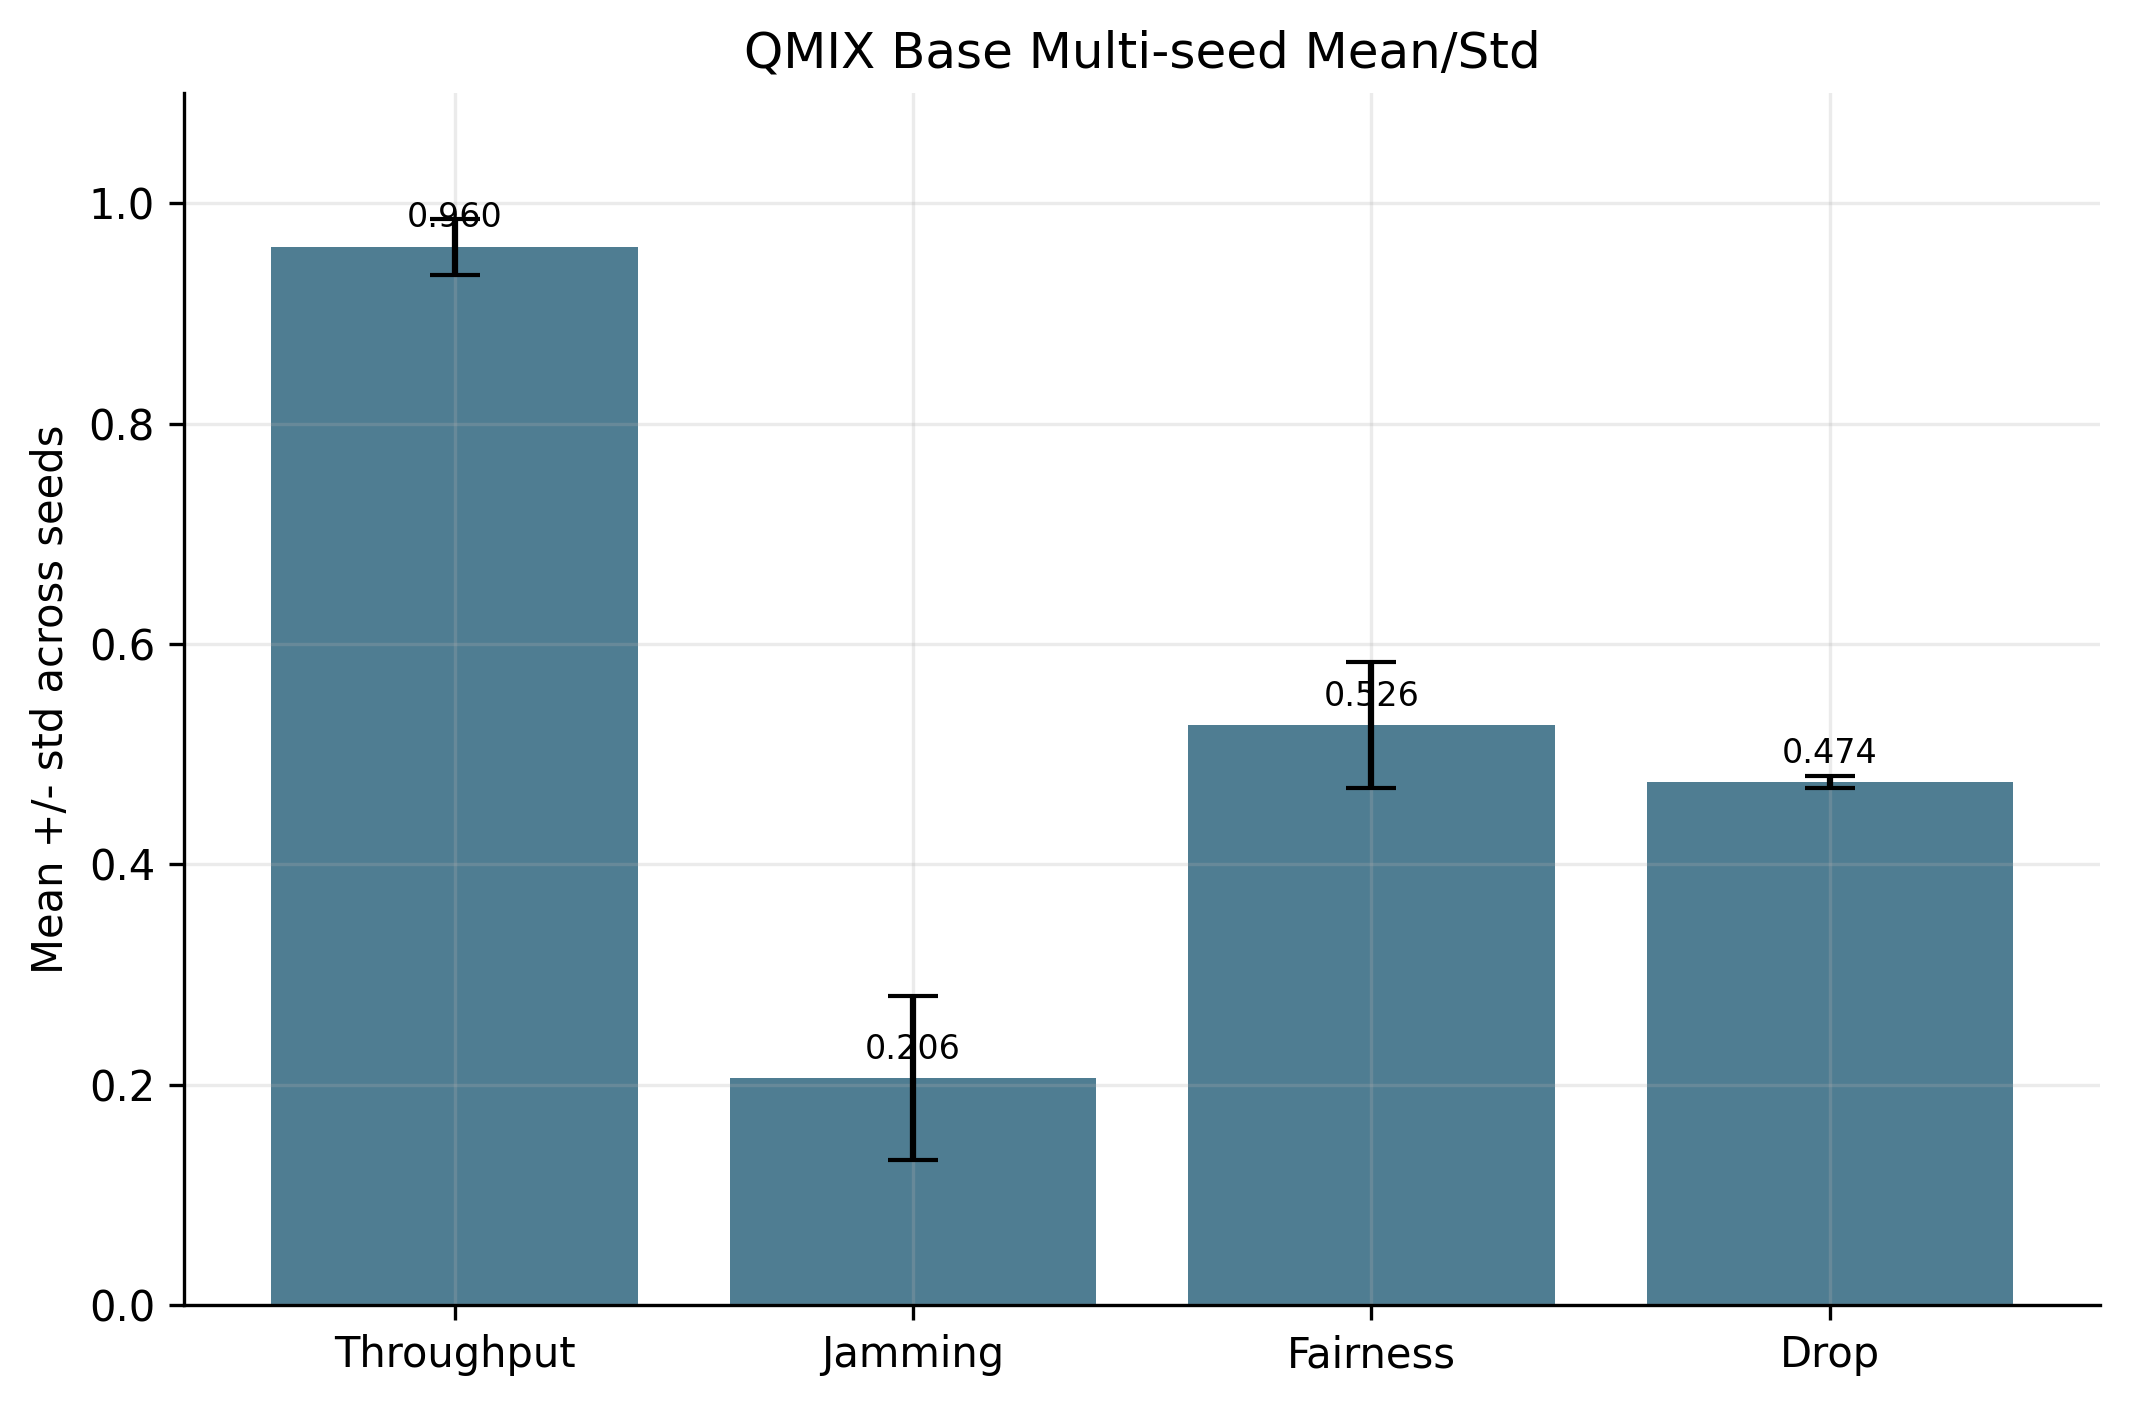
\includegraphics[width=0.82\textwidth]{fig4_qmix_multiseed_mean_std.png}
\caption{Mean/std của QMIX base trên ba seed. Throughput ổn định hơn so với các chỉ số phối hợp như jamming failure và fairness.}
\label{fig:qmix_multiseed}
\end{figure}

Số seed là ba nên kết luận về thống kê cần thận trọng. Tuy nhiên, trong phạm vi này, QMIX base duy trì thông lượng cao và có jamming failure thấp hơn Hierarchical DDQN đơn chạy.

\section{Ablation công bằng}

Bảng \ref{tab:fairness_ablation} và Hình \ref{fig:fairness_tradeoff} cho thấy các biến thể fairness. Biến thể fair\_w2 cải thiện throughput và jam nhưng giảm fairness trung bình xuống \(0.5111\pm0.1478\). Biến thể fair\_w3 làm giảm throughput và không cải thiện fairness. Do đó, tăng trọng số fairness trong executor không tự động tạo trade-off tốt hơn.

\begin{table}[H]
\centering
\caption{Ablation công bằng. QMIX base được giữ làm thiết lập cuối cùng vì trade-off tổng thể tốt nhất trong các biến thể đã kiểm tra.}
\label{tab:fairness_ablation}
\scriptsize
\resizebox{\textwidth}{!}{\begin{tabular}{llllll}
\hline
Variant & Throughput/frame mean +/- std & Drop mean +/- std & Jamming failure mean +/- std & Fairness mean +/- std & Interpretation \\
\hline
QMIX base & 0.9604 +/- 0.0255 & 0.4744 +/- 0.0054 & 0.2056 +/- 0.0744 & 0.5260 +/- 0.0572 & Best overall trade-off; final MaDRL setting. \\
fair\_w2 & 0.9883 +/- 0.0350 & 0.4771 +/- 0.0180 & 0.1601 +/- 0.0501 & 0.5111 +/- 0.1478 & Improves throughput and jamming but reduces mean fairness. \\
fair\_w3 & 0.8877 +/- 0.0094 & 0.4938 +/- 0.0113 & 0.3123 +/- 0.0711 & 0.4933 +/- 0.1880 & Excessive fairness weighting degrades performance. \\
no\_balance\_action & 0.8439 +/- 0.0473 & 0.4926 +/- 0.0065 & 0.3352 +/- 0.0598 & 0.4767 +/- 0.0401 & Disabling balance action hurts fairness, throughput, and jamming. \\
\hline
\end{tabular}
}
\end{table}

\begin{figure}[H]
\centering
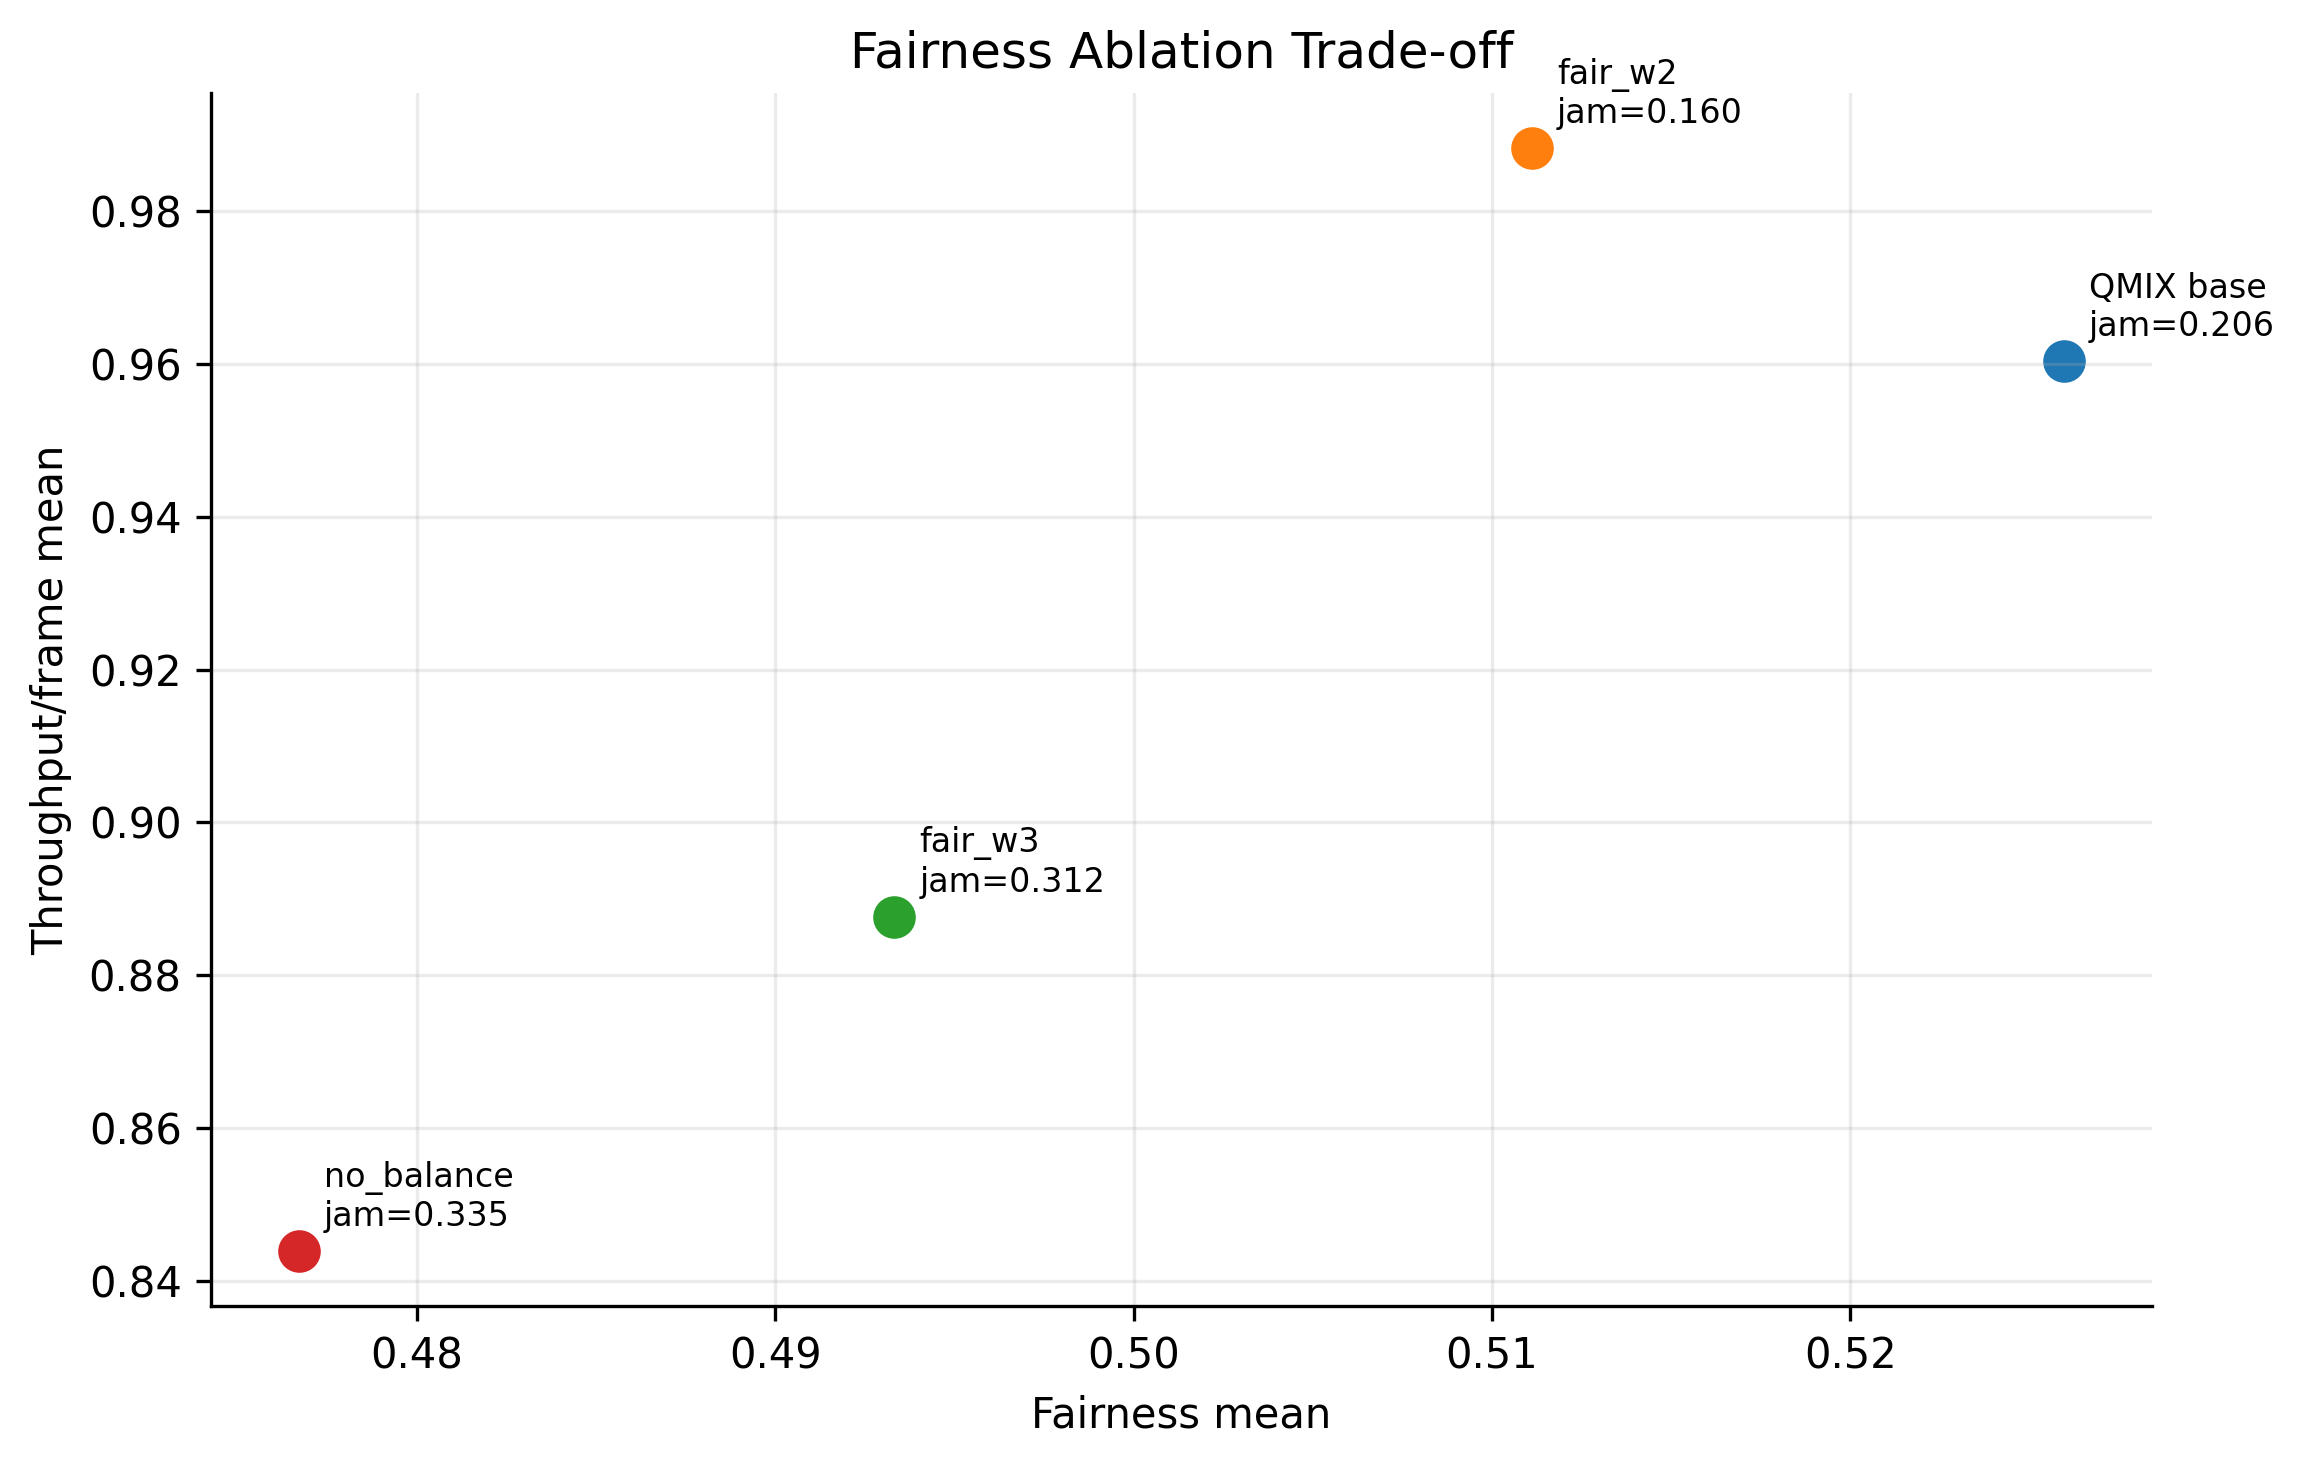
\includegraphics[width=0.82\textwidth]{fig5_fairness_ablation_tradeoff.png}
\caption{Đánh đổi throughput--fairness trong các biến thể. fair\_w2 có throughput và jamming tốt hơn nhưng fairness trung bình thấp hơn QMIX base.}
\label{fig:fairness_tradeoff}
\end{figure}

\begin{figure}[H]
\centering
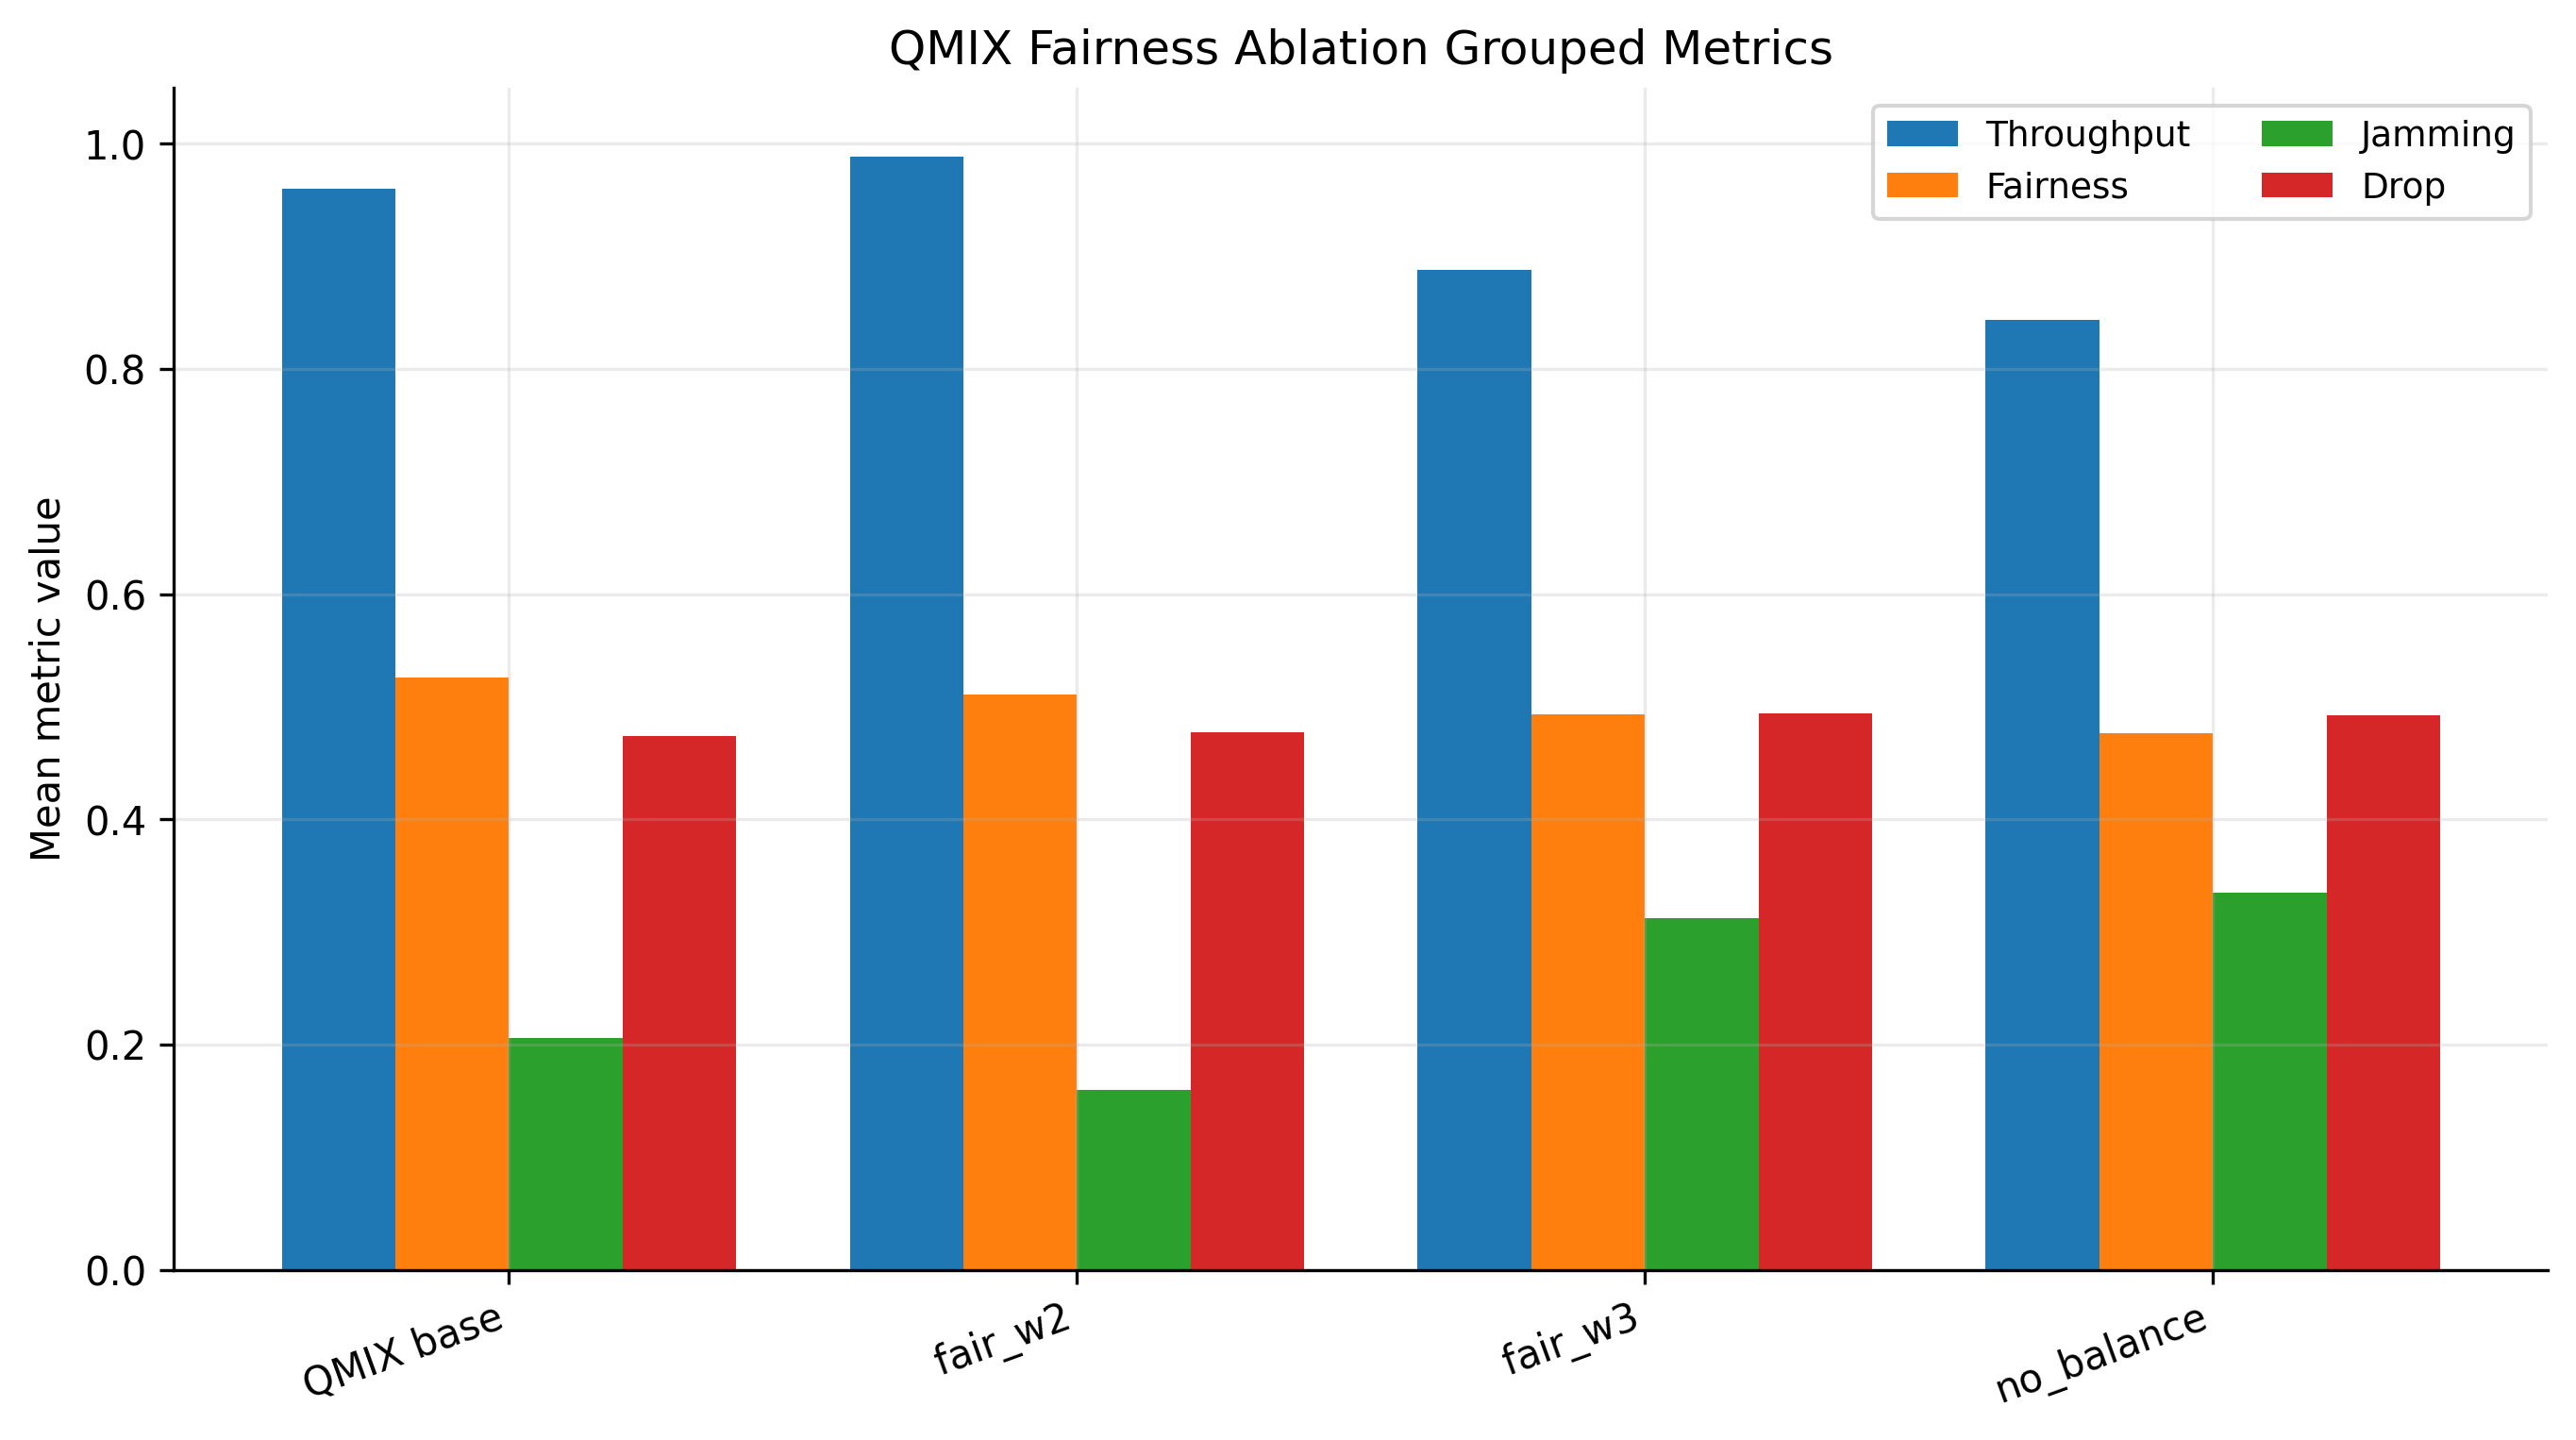
\includegraphics[width=0.88\textwidth]{fig6_fairness_ablation_bars.png}
\caption{Ablation công bằng theo nhóm chỉ số. Vô hiệu hóa hành động cân bằng làm giảm throughput/fairness và tăng jamming so với QMIX base.}
\label{fig:fairness_bars}
\end{figure}

Biến thể no\_balance\_action đạt throughput \(0.8439\pm0.0473\), fairness \(0.4767\pm0.0401\) và jam \(0.3352\pm0.0598\), đều kém hơn QMIX base. Điều này ủng hộ vai trò của BALANCE\_UNDERSERVED\_IOT như một thành phần hỗ trợ phối hợp công bằng, nhưng không có nghĩa fairness đã được giải quyết hoàn toàn.

\section{Thảo luận}

Kết quả hỗ trợ ba điểm chính. Một là Flat DDQN gặp khó với giao diện hành động 864 chiều. Hai là trừu tượng hóa hành động 10 mức cao là bước cải thiện quyết định. Ba là QMIX-Hierarchical cung cấp cấu trúc học hợp tác phù hợp hơn cho nhiều UAV, đặc biệt ở các chỉ số jamming/fairness.

Các giới hạn phải được giữ rõ. Kết quả dựa trên mô phỏng với 2 UAV, 15 IoT và 1 jammer. Backscatter là abstraction mức hệ thống. Executor là rule-based và dùng thông tin môi trường. Một số baseline là kết quả đơn chạy, trong khi QMIX có đánh giá ba seed. Không có xác thực phần cứng và không có huấn luyện lại trong giai đoạn viết báo cáo.

\section{Kết luận}

Báo cáo đã trình bày bài toán điều khiển UAV-IoT dưới jammer di động với truyền thông backscatter-inspired/RF-powered ở mức hệ thống. Kết quả cho thấy Flat DDQN không đủ mạnh trong Scenario 4 do không gian hành động nguyên thủy lớn. Giao diện hành động phân cấp giảm số hành động trực tiếp từ 864 xuống 10 và giúp DDQN học được chính sách hiệu quả hơn. Trên cơ sở đó, QMIX-Hierarchical được chọn làm phương pháp MaDRL cuối cùng nhờ khả năng phối hợp nhiều UAV với quan sát cục bộ, phần thưởng chung, action masking và mixer dùng trạng thái toàn cục.

Kết luận cần được hiểu trong phạm vi mô phỏng hiện tại. QMIX-Hierarchical không được khẳng định là vượt Hierarchical DDQN về throughput trung bình, nhưng có bằng chứng tốt hơn về ổn định đa seed và cải thiện trade-off gây nhiễu/công bằng. Fairness còn ở mức trung bình và cần nghiên cứu tiếp.

\section{Hướng phát triển}

Các hướng phát triển tiếp theo gồm:

\begin{itemize}
  \item mở rộng quy mô với nhiều UAV, nhiều IoT và nhiều jammer hơn;
  \item kiểm tra jammer thông minh hơn, thích nghi theo chính sách UAV hoặc có chiến lược gây nhiễu học được;
  \item cải thiện mô hình vật lý backscatter, bao gồm liên kết RF-source--IoT--UAV và điều kiện phần cứng thực tế;
  \item thay executor rule-based bằng executor học được hoặc chính sách phân cấp end-to-end;
  \item thiết kế mục tiêu fairness mạnh hơn, ví dụ reward shaping theo per-IoT service gap hoặc constrained RL;
  \item chạy thêm seed, kiểm định thống kê và ablation rộng hơn;
  \item đánh giá trên môi trường thực nghiệm hoặc hardware-in-the-loop.
\end{itemize}


\clearpage
\bibliographystyle{plainnat}
\bibliography{references}

\end{document}
